\documentclass[12pt,a4paper]{book}

% Add preamble
% Language and encoding
\usepackage[utf8]{inputenc}
\usepackage[T1]{fontenc}
\usepackage[brazil]{babel}

% Additional commands to math mode
\usepackage{amsmath}

% Indent first line of first paragraph
\usepackage{indentfirst}

% Page numbering
\pagestyle{empty}

% Don't put page number on empty page
\usepackage{emptypage}

% Hypertext references
% \usepackage{hyperref}

% Remove space after a comma when it acts like a decimal separator
\usepackage{icomma}

% Enable use of colours
\usepackage[usenames,svgnames,dvipsnames]{xcolor}

% Show customised enumerate
\usepackage{enumerate}

% Support graphics
\usepackage[pdftex]{graphicx}

% Input raw text
\usepackage{verbatim}

% Include external raw PDF pages
\usepackage{pdfpages}

% Allow forcing a figure to be displayed "here"
\usepackage{float}

% Input code
\usepackage{listings} \lstset{basicstyle=\ttfamily}


% ---------------------------------------------------------------------
% Additional packages

\usepackage{setspace}    % Flexible spacing
\usepackage{makeidx}     % Index
\usepackage{tocbibind}   % Add bibliography/index/content to ToC
\usepackage{courier}     % Adobe Courier instead of Computer Modern Typewriter
\usepackage{type1cm}     % Scalable fonts
\usepackage{titletoc}
\usepackage[fixlanguage]{babelbib}
\usepackage[font=small,format=plain,labelfont=bf,up,textfont=it,up]{caption}

% Margins
\usepackage[a4paper,top=3cm,bottom=2cm,inner=2cm,outer=2cm]{geometry}

% Solve hyperref and chapter problem
\usepackage[all]{hypcap}

% Textual bibliography quote
\usepackage[round,sort,nonamebreak]{natbib}

% Disable hyphenation of some words
% Disable hyphenation on following words

\hyphenation{game}
\hyphenation{games}
\hyphenation{engine}
\hyphenation{engines}
\hyphenation{software}

\hyphenation{Cambridge}
\hyphenation{University}
\hyphenation{Engineering}
\hyphenation{Department}
\hyphenation{Carnegie}
\hyphenation{Mellon}

\hyphenation{CMUSphinx}
\hyphenation{Sphinxbase}
\hyphenation{Pocketsphinx}
\hyphenation{Speech}
\hyphenation{Text}
\hyphenation{utterance}
\hyphenation{utterances}
\hyphenation{senone}
\hyphenation{senones}
\hyphenation{Hidden}
\hyphenation{Markov}
\hyphenation{Model}
\hyphenation{sinal/ruído}

\hyphenation{Windows}
\hyphenation{MacOS}
\hyphenation{Unix}
\hyphenation{Linux}
\hyphenation{Ubuntu}
\hyphenation{Debian}
\hyphenation{Android}
\hyphenation{iOS}

\hyphenation{Godot}
\hyphenation{GDScript}
\hyphenation{script}
\hyphenation{scripts}
\hyphenation{object}
\hyphenation{objects}
\hyphenation{reference}
\hyphenation{references}
\hyphenation{resource}
\hyphenation{resources}
\hyphenation{node}
\hyphenation{nodes}
\hyphenation{scene}
\hyphenation{scenes}

\hyphenation{getter}
\hyphenation{getters}
\hyphenation{setter}
\hyphenation{setters}
\hyphenation{thread}
\hyphenation{threads}

\hyphenation{STTConfig}
\hyphenation{STTRunner}
\hyphenation{STTQueue}
\hyphenation{STTError}
\hyphenation{FileDirUtil}

\hyphenation{Color}
\hyphenation{Clutter}
\hyphenation{background}
\hyphenation{start}
\hyphenation{running}
\hyphenation{exit}


% Add metadata to PDF
\hypersetup{
    pdfauthor = {Leonardo Pereira Macedo},
    pdftitle = {Desenvolvimento de um módulo para Godot},
    pdfsubject = {Trabalho de Conclusão de Curso - IME-USP},
    pdfkeywords = {software, game engine, Godot, desenvolvimento de módulo,
                   reconhecimento de voz},
    pdfpagemode = UseOutlines
}

\fontsize{60}{62}\usefont{OT1}{cmr}{m}{n}{\selectfont}

% Paragraph indent size
% \setlength{\parindent}{2cm}

% Spacing between paragraphs
% \setlength{\parskip}{0.25cm}

% ---------------------------------------------------------------------
% Nice headers

\usepackage{fancyhdr}
\pagestyle{fancy}
\fancyhf{}

\renewcommand{\chaptermark}[1]{\markboth{\MakeUppercase{#1}}{}}
\renewcommand{\sectionmark}[1]{\markright{\MakeUppercase{#1}}{}}
\renewcommand{\headrulewidth}{1pt}

% Display centered page number on footer of all pages
\fancyfoot[CE,CO]{\thepage}

% Fix headheight to avoid warnings
\setlength{\headheight}{15pt}

% ---------------------------------------------------------------------

\urlstyle{same}  % URL with same style as text and not monospaced
\makeindex
\raggedbottom    % Disallow extra spaces in text
\fontsize{60}{62}\usefont{OT1}{cmr}{m}{n}{\selectfont}
\cleardoublepage
\normalsize

% =====================================================================
% Document initial pages

\begin{document}
\sloppy  % Prevents words from passing line length

\frontmatter
\setcounter{tocdepth}{2}

% Header for pages in sections before chapter 1
\fancyhead[RO]{\nouppercase{\rightmark}}
\fancyhead[LE]{\nouppercase{\leftmark}}
\fancyhead[RE,LO]{}

\linespread{1.25}

\pagenumbering{gobble}
\hypersetup{pageanchor=false}
\thispagestyle{empty}
\begin{center}
    \vspace*{2.3cm}
    Universidade de São Paulo \\
    Instituto de Matemática e Estatística \\
    Bachalerado em Ciência da Computação


    \vspace*{3cm}
    \large{Leonardo Pereira Macedo}


    \vspace{3cm}
    \textbf{\large{Desenvolvimento de um módulo de reconhecimento de voz \\
    para a \textit{game engine} \textit{Godot}}}


    \vskip 5cm
    \normalsize{São Paulo}

    \today
\end{center}

\newpage
\thispagestyle{empty}
  \begin{center}
    \vspace*{2.3 cm}
    \textbf{\Large{Desenvolvimento de um plugin\\
    para a \textit{game engine} Godot}}
    \vspace*{2 cm}
  \end{center}

  \vskip 2cm

  \begin{flushright}
    Monografia final da disciplina\\
    MAC0499 -- Trabalho de Formatura Supervisionado
  \end{flushright}

  \vskip 5cm

  \begin{center}
  Supervisor: Prof. Dr. Marco Dimas Gubitoso\\

  \vskip 5cm
  \normalsize{São Paulo}

  \today
  \end{center}
\pagebreak

\pagenumbering{roman}  % Begin enumerating


\hypersetup{pageanchor=true}
\pagenumbering{roman}
\onehalfspacing
% ---------------------------------------------------------------------
% Portuguese

\chapter*{Resumo}

A área de \emph{games} evoluiu muito desde o início da década da 70, quando começaram
a ser comercializados. As principais causas estão relacionadas aos avanços em
diferentes áreas da Computação.

Com o passar do tempo, surgiram as \emph{game engines}: \emph{frameworks} voltados
especificamente para a criação de jogos, visando a facilitar o desenvolvimento e/ou
algumas de suas etapas.

Focaremos em uma \emph{game engine} em particular, \emph{Godot}. Por possuir código
aberto, este \emph{software} permite a extensão de suas funcionalidades através da
criação de novos módulos.

Este projeto busca implementar um módulo de reconhecimento de voz para \emph{Godot},
depois demonstrando a nova capacidade em um jogo simples desenvolvido na própria
plataforma.
\\

\noindent \textbf{Palavras-chave:} \emph{software}, \emph{game engine}, \emph{Godot},
desenvolvimento de módulo, extensão de funcionalidade.

% ---------------------------------------------------------------------
% English

\chapter*{Abstract}

Video games have evolved considerably since the beginning of the 70's, when they
started to be commercialized. The main reasons are related to several advances in
different fields of Computer Science.

Over time, \emph{game engines} started appearing: \emph{frameworks} designed
specifically to assist on game creation, simplifying the process and/or some of its
steps.

We will focus on a specific game engine, \emph{Godot}. Since it is an open source
project, it is possible to extend its funcionalities by creating new modules.

This project's goal is to implement a speech recognition module for \emph{Godot},
then showing the new feature in a simple game developed on the engine itself.
\\

\noindent \textbf{Keywords:} software, game engine, \emph{Godot}, module development,
functionality extension.


% Add list of listings to ToC
\renewcommand{\lstlistoflistings}{
\begingroup
\tocfile{\lstlistlistingname}{lol}
\endgroup
}

{
\hypersetup{linkcolor=black}
\tableofcontents
\listoffigures
\listoftables
\lstlistoflistings
}

% ---------------------------------------------------------------------
% Document main body

\mainmatter
\pagenumbering{arabic}

% Header for all pages in chapters
\fancyhead[LE,RO]{\footnotesize\thesection\quad\nouppercase{\rightmark}}
\fancyhead[RE,LO]{\chaptername\:\thechapter:\quad\nouppercase{\leftmark}}

% Add chapters here
\chapter{Introdução}
\label{cap:introduction}

% ---------------------------------------------------------------------

\section{Motivação e objetivo}

Hoje em dia, não há como negar que o mercado de \textit{games} é um fenômeno mundial, gerando mais de US\$ 91 bilhões em 2016 \citep{gameMarket:16}. Comparado aos primeiros jogos, comercializados no início da década de 1970 \citep{gameMarketOrigin}, a evolução em diversas áreas da computação permitiu grandes avanços nos jogos criados. Inclui-se nisso a evolução dos computadores por conta da \textit{Lei de Moore} \citep{moore}, permitindo processamento mais rápido; \textit{games} em 3D e gráficos cada vez mais sofisticados e realistas devido à Computação Gráfica; e adversários sofisticados e de raciocínio rápido com a Inteligência Artificial.

Junto aos próprios jogos, as tecnologias usadas para desenvolvê-los também tiveram progressos. Em especial, temos as \emph{game engines}, que podem ser descritas como \textquotedblleft \textit{frameworks} voltados especificamente para a criação de jogos\,\textquotedblright\:\citep{gameEngine:13}. Elas oferecem diversas ferramentas para acelerar o desenvolvimento de um jogo, como maior facilidade na manipulação gráfica e bibliotecas prontas para tratar colisões entre objetos. Além disso, como eficiência é um fator essencial para manter um bom valor de FPS (\textit{Frames per Second}), as \textit{engines} costumam ter sua base construída em linguagens rápidas e compiladas, como C e C++.

Focaremos em uma \textit{game engine} em particular, \textbf{\emph{Godot}} \citep{godot}. O principal motivo de ter sido escolhida é por ser um \textit{software} de código aberto, o que permite a qualquer pessoa baixar seu código fonte e fazer modificações. Em especial, a \textit{engine} permite a criação de novos módulos para adicionar a ele novas funcionalidades.

Este trabalho visa a criar um novo módulo para \textit{Godot}. Tal extensão adicionará funções simples de reconhecimento de voz, algo ainda inexistente no \textit{software}. Feito isso, a nova funcionalidade será demonstrada em um jogo simples criado nessa \textit{engine}.

% ---------------------------------------------------------------------

\section{Organização do trabalho}

O capítulo \ref{cap:speech-recognition} aborda resumidamente reconhecimento de voz através de um olhar teórico, seguido pelo capítulo \ref{cap:hmm}, onde estuda-se um pouco de uma forma de realizar reconhecimento de voz por meio de \textit{Modelos Ocultos de Markov}.

No capítulo \ref{cap:speech-libs}, representa-se os primeiros passos para a concretização do trabalho, pois envolve a busca da melhor biblioteca de reconhecimento de voz que possa ser usada no módulo. A biblioteca escolhida, \textit{Pocketsphinx}, é estudada no capítulo \ref{cap:pocketsphinx}.

A arquitetura do \textit{Godot} é apresentada no capítulo \ref{cap:godot} a fim de se entender a lógica por trás da construção do módulo de reconhecimento de voz no capítulo \ref{cap:stt-module}. O capítulo \ref{cap:color-clutter} apresenta a criação de jogo simples, feito na própria \textit{game engine}, para demonstrar o módulo em funcionamento e suas capacidades.

% TODO: Check where the subjective chapters will be placed
O capítulo \ref{cap:conclusion} apresenta as conclusões do trabalho. Por fim, há uma parte subjetiva contendo a apreciação pessoal do TCC e uma descrição das matérias que mais ajudaram no desenvolvimento do projeto.

\chapter{Reconhecimento de voz}
\label{cap:speech-recognition}

Neste capítulo, abordaremos a parte teórica do reconhecimento de voz, sem nos preocuparmos com a forma de implementação ou sua aplicação no contexto deste trabalho. Em particular, analisaremos brevemente os principais parâmetros que influenciam seu uso.

% ---------------------------------------------------------------------

\section{Definição}

\textbf{Reconhecimento automático de voz} (ou da fala), muitas vezes referido como \textit{speech to text} (\textbf{STT}) ou \textit{automatic speech recognition} (\textbf{ASR}), é um campo multidisciplinar que envolve as áreas de Inteligência Artificial, Estatística e Linguística. Busca-se desenvolver metodologias e tecnologias para que computadores sejam capazes de captar, reconhecer e traduzir a linguagem falada para texto \citep{sttDefinition}.

% ---------------------------------------------------------------------

\section{História}

Apresentamos uma breve visão histórica de sistemas de reconhecimento de voz, desde seu início até os dias atuais. Baseamo-nos principalmente em um artigo \citep{STTHistory}.

% ---------------------------------------------------------------------

\subsection{Décadas de 50 e 60: Primeiros passos}

O primeiro sistema de reconhecimento de voz conhecido foi o \textit{Audrey}, construído em 1952 por três pesquisadores do \textit{Bell Labs}. A máquina conseguia reconhecer apenas dígitos falados por um único usuário.

10 anos depois, a IBM apresentou o \textit{Shoebox}, que reconhecia 16 palavras em inglês, entre elas os dígitos de 0 a 9. Quando captava palavras como \textit{plus}, \textit{minus} ou \textit{total}, \textit{Shoebox} instruía outra máquina de adições a realizar cálculos ou imprimir o resultado. A entrada era feita por um microfone (figura \ref{shoebox}), que convertia a voz do usuário em impulsos elétricos, classificados internamente por um circuito de medição \citep{shoebox}.

\begin{figure}[H]
  \centering
  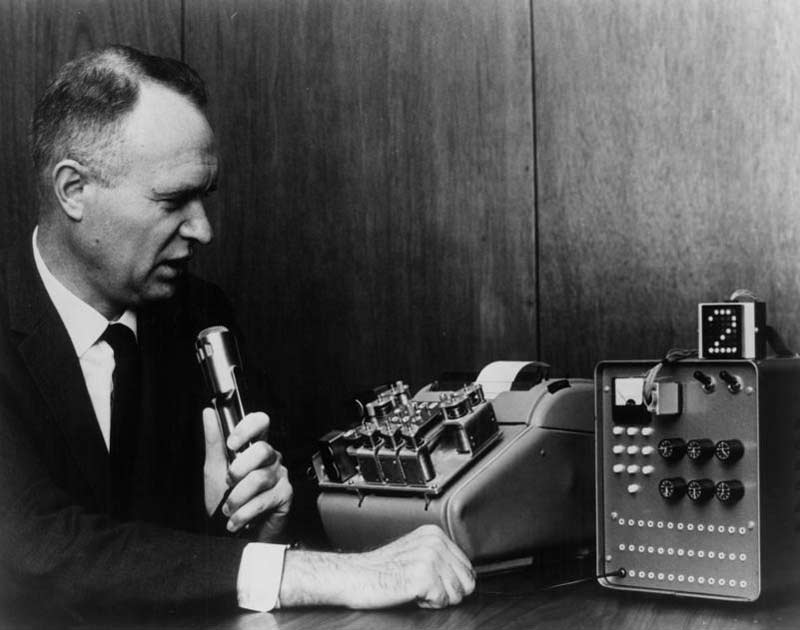
\includegraphics[width=.5\textwidth]{image/shoebox.jpg}
  \caption{Máquina \textit{Shoebox} sendo operada \citep{shoeboxImage}}
  \label{shoebox}
\end{figure}

Laboratórios nos EUA, URSS, Inglaterra e Japão começaram a desenvolver \textit{hardware} para reconhecer uma maior variedade de sons. Conseguiu-se suporte para quatro vogais e nove consoantes; um avanço notável, considerando a tecnologia da época.

% ---------------------------------------------------------------------

\subsection{Décadas de 70 e 80: Grandes avanços}

Na década de 70, o departamento de defesa dos EUA mostrou grande interesse em financiar a tecnologia de reconhecimento de voz. Tal impulso ajudou no desenvolvimento do sistema \emph{Harpy} de reconhecimento de voz pela Universidade Carnegie Mellon.

\textit{Harpy} usava um grafo para representar o domínio das palavras reconhecíveis. Um algoritmo de busca heurística, \emph{Beam Search}, era aplicado para procurar a melhor interpretação para a voz de entrada. Este algoritmo assemelha-se ao \textit{Best-First Search} (BFS), que explora um grafo através da expansão do estado mais promissor ao sair do estado presente. No entanto, sua otimização consiste em ordenar os próximos possíveis estados, através de uma heurística, antes de realizar uma expansão, o que permite prever o quão longe o estado presente está em relação ao estado meta. Com isso, o \textit{Beam Search} é caracterizado como um algoritmo guloso, que gasta menos memória quando comparado ao BFS \citep{beamSearch}.

Através de uma forma de busca mais eficiente, \textit{Harpy} conseguia entender 1011 palavras, aproximadamente o vocabulário de uma criança típica de três anos.

Sistemas de reconhecimento de voz só tiveram um avanço realmente significativo na década de 80, devido a um método estatístico denominado \textbf{Modelo Oculto de Markov} (ou \textbf{HMM}, sigla para \textit{Hidden Markov Model}). Ao invés de procurar por modelos de palavras em padrões de som, considera-se a probabilidade de um som desconhecido possuir palavras, o que acelerou o processo e tornou possível usar um vocabulário maior nos computadores.\iffalse Veremos HMM com mais detalhes no capítulo \ref{cap:hmm}.\fi

Outro modelo que ganhou bastante popularidade na mesma época foi o de redes neurais, que é efetivo para classificar palavras isoladas e fonemas individuais mas encontra problemas em tarefas envolvendo reconhecimento contínuo. Ao contrário do HMM, este método não consegue modelar bem dependências temporais. No entanto, em ambos os casos, existia a necessidade de falar pausadamente para o sistema poder melhor interpretar o usuário.

Os progressos em sistemas de reconhecimento de voz começaram a se refletir no meio comercial. Destacamos a boneca \textit{Julie} (figura \ref{julie}), comercializada em 1987 como \textit{``Finalmente, a boneca que te entende''}, pois era capaz de ser treinada para responder à voz de uma criança.

\begin{figure}[H]
  \centering
  
\includegraphics[width=.35\textwidth]{image/julie.jpg}
  \caption{Caixa da boneca \textit{Julie}; note, na parte inferior, a frase \textit{``Ela entende o que você diz''} \citep{julieImage}}
  \label{julie}
\end{figure}

% ---------------------------------------------------------------------

\subsection{Década de 90 até hoje: Popularização}

Na década de 90, a popularização de computadores para uso pessoal e o desenvolvimento de processadores mais rápidos permitiu que o reconhecimento de voz ficasse viável para uma quantidade maior de pessoas.

Em 1996, surgiu o primeiro portal de voz, VAL, criado pela empresa de telecomunicações norte-americana BellSouth. O sistema atendia chamadas telefônicas e respondia de acordo com a informação proferida pelo cliente.

Até o final dos anos 2000, sistemas de reconhecimento de voz pareciam ter ficado estagnados em uma acurácia de aproximadamente 80\%, e muitas aplicações eram caracterizadas pela complexidade ou dificuldade de uso se comparadas ao tradicional \textit{mouse} e teclado.

A popularidade do conceito ressurgiu com força através do aplicativo de Busca por Voz, feito pela Google para \textit{iPhone}. As duas razões para tal sucesso eram a facilidade de entrada de dados, se comparado ao teclado da plataforma, e o uso de \textit{data centers} em nuvem da Google, o que retirava a necessidade de um poderoso processamento nos \textit{iPhones} em si. Com isso, mostrava-se que era possível contornar duas das principais limitações de sistemas de voz: a disponibilidade de dados e a dificuldade de processá-los eficientemente.

A evolução na tecnologia de reconhecimento de voz foi tamanha que, atualmente, é inegável seu impacto em nosso dia a dia. Um celular moderno consegue captar palavras ou pequenas frases de seu usuário dentre um enorme vocabulário para fazer buscas na Internet, tocar uma música ou fazer uma ligação. Alguns países usam reconhecimento de voz para autenticar a identidade de alguém por telefone, com o objetivo de evitar fornecer dados pessoais pelo mesmo. Também há usos em transportes, na área médica e para fins educativos, muitas vezes acentuados pela maior facilidade em se falar um comando comparado ao uso de um teclado ou interface gráfica.

% ---------------------------------------------------------------------

\section{Componentes de um sistema genérico}
\label{sttComponents}

A figura \ref{generic-stt} apresenta os três componentes de um sistema genérico envolvendo STT \citep{sttComponentsParameters}:

\begin{itemize}
\item O \textbf{usuário} do sistema, que codifica um comando através de sua voz;

\item O \textbf{dispositivo} de STT, que converte a mensagem falada para um formato interpretável;

\item O \textbf{software de aplicação}, que recebe a saída do dispositivo e realiza uma ação apropriada.
\end{itemize}

\begin{figure}[H]
  \centering
  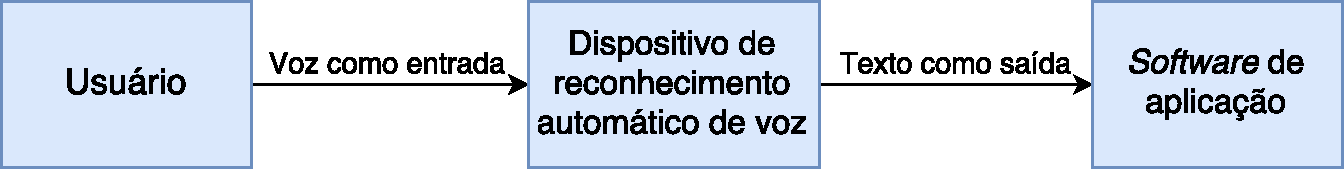
\includegraphics[width=.9\textwidth]{image/generic-stt.pdf}
  \caption{Sistema genérico de reconhecimento automático de voz \citep{sttComponentsParameters}}
  \label{generic-stt}
\end{figure}

% ---------------------------------------------------------------------

\section{Principais termos}
\label{sttMainTerms}

De acordo com \citep{sttComponentsParameters} e \citep{sttBasics}, apresentamos, a seguir, os termos mais recorrentes em sistemas de reconhecimento de voz. Também detalhamos seus parâmetros principais, que atuam sobre sua forma de funcionamento, eficiência e acurácia. A influência destes fatores varia de acordo com o tipo de aplicação que se deseja construir.

% ---------------------------------------------------------------------

\subsection{Fluência}

A fluência está relacionada à forma de se comunicar com o sistema. Tipicamente, a fala do usuário pode ser feita através de:

\begin{itemize}
\item \textbf{Palavras isoladas}, com pausas entre elas;
\item \textbf{Palavras conectadas}, que são concatenadas sem pausas;
\item \textbf{Fala contínua}, onde o fluxo de palavras é semelhante a uma fala natural.
\end{itemize}

% ---------------------------------------------------------------------

\subsection{Dependência do usuário}

A dependência ou não do usuário classifica os sistemas em dois grupos:

\begin{itemize}
\item Os sistemas \textbf{dependentes} (\textit{speaker-dependent}), caracterizados pelo \emph{treinamento} feito pelo usuário. Isto é, são computadores que analisam e se adaptam aos padrões particulares da fala captada, resultando em uma maior acurácia. Geralmente, o usuário deve ler algumas páginas de texto para a máquina antes de iniciar o uso do sistema. Esta variante é comumente escolhida em casos particulares, onde um número limitado de palavras deve ser reconhecido com bastante precisão \citep{speakerDependency}.

\item Os sistemas \textbf{independentes} (\textit{speaker-independent}), que são desenvolvidos para reconhecer a voz de qualquer pessoa e não requerem treinamento. É a melhor opção para aplicações interativas que usam voz, já que não é viável fazer com que os usuários leiam páginas de texto antes do uso, ou para sistemas usados por diferentes pessoas. Sua desvantagem é a acurácia menor se comparado ao reconhecimento dependente; para contornar isso, costuma-se limitar o vocabulário reconhecido pelo sistema \citep{speakerDependency}.
\end{itemize}

% ---------------------------------------------------------------------

\subsection{Vocabulário}

O vocabulário representa as palavras reconhecidas pelo sistema. Seu tamanho pode ser pequeno (menor que 20 palavras) até muito grande (mais de 20 mil palavras), sendo diretamente proporcional à velocidade do reconhecimento. Além disso, a similaridade entre a pronúncia de algumas palavras pode afetar a acurácia, uma vez que a distinção entre elas torna-se mais complicada.

% ---------------------------------------------------------------------

\subsection{\textit{Utterance}}

O termo \textit{utterance} não possui uma tradução exata no contexto de reconhecimento de voz, embora possa ser interpretado como \textit{``pronunciamento, elocução''}. Refere-se à vocalização (fala) de uma ou mais palavras, pronunciadas de forma contínua e terminando com uma pausa clara, que possuem um significado único ao computador. Em outras palavras, \textit{utterances} são o conteúdo entendido pelo sistema após receber a fala do usuário.

Ao voltarmos para o sistema genérico de reconhecimento de voz apresentado na seção \ref{sttComponents}, notaremos que a interpretação de \textit{utterances} representa a saída produzida pelo dispositivo de STT.

% ---------------------------------------------------------------------

\subsection{Taxa de erro por palavra}
\label{word-error-rate}

A taxa de erro por palavra (\textit{word error rate}, ou $WER$) é uma métrica de desempenho de um sistema de reconhecimento de voz \citep{wordErrorRate}.

Suponha que tenhamos o texto de referência $\tau$, correspondente ao que o usuário falou, e o texto $\tau'$ de hipótese, que foi gerado pelo sistema STT. O reconhecimento de voz pode levar a diferentes interpretações nas $N$ palavras de $\tau$, levando a um $\tau'$ diferente. Em particular, costuma haver um certo número $I$ de palavras inseridas, uma quantidade $D$ de palavras removidas e um valor $S$ de palavras substituídas.

Exemplificando, seja $\tau$ = \textit{``Gosto de chocolate''} e $\tau'$ = \textit{``Gosto chocolate''}. Houve uma remoção por conta da preposição \textit{``de''} ter sido eliminada pelo sistema de reconhecimento de voz, então $D = 1$.

A taxa de erro $WER$, geralmente expressa como uma porcentagem, é dada pela equação \ref{wer-equation}. Um valor elevado para esta métrica significa que a qualidade do reconhecimento de voz está ruim.

\begin{equation}
\label{wer-equation}
WER =  \frac{I + D + S}{N}
\end{equation}

% ---------------------------------------------------------------------

\subsection{Parâmetros ambientais}

Parâmetros ambientais referem-se a fatores externos ao sistema que podem interferir no reconhecimento de voz. Destacam-se:

\begin{itemize}
\item A \textbf{relação sinal/ruído}, que avalia a intensidade média do sinal recebido em relação ao ruído de fundo, tipicamente medido em decibéis (dB). Quanto menor a taxa, maior a dificuldade no reconhecimento de voz.

\item O \textbf{próprio usuário}, o que inclui o volume de sua voz, a velocidade com que fala e até mesmo sua condição psicológica: o nível de estresse de um piloto sob ataque em uma aeronave é diferente de alguém simplesmente querendo ouvir uma música, por exemplo.
\end{itemize}

% \chapter{Modelo Oculto de Markov}
\label{cap:hmm}

\chapter{Bibliotecas para Reconhecimento de Voz}
\label{cap:speech-libs}

A seguir, veremos o primeiro item necessário para atingirmos o objetivo final: uma biblioteca que fará o reconhecimento de voz dentro do módulo.

Uma implementação do zero fugiria do tema deste trabalho, pois seria necessário aprender sobre reconhecimento de padrões voltado a sons e outros tópicos relacionados a Inteligência Artificial. A outra opção existente, e a que seguiremos, é procurar por uma biblioteca existente e aprender a manejá-la.

Analisaremos quais as características necessárias e desejáveis na biblioteca ideal, e estudaremos a que melhor se adequa ao nosso objetivo dentre as opções existentes.

% ---------------------------------------------------------------------

\section{Considerações iniciais}

Recordemos os principais componentes para reconhecimento de voz, apresentados na seção \ref{sttComponents}. No contexto do módulo de reconhecimento de voz para \textit{Godot}, as seguintes associações surgem naturalmente:

\begin{itemize}
\item O \textbf{usuário} representa tipicamente o \textbf{jogador}, que interage parcialmente ou totalmente com o jogo por meio de comandos de voz.

\item O \textbf{dispositivo de STT} corresponde ao \textbf{módulo de reconhecimento de voz}, objetivo principal deste trabalho. Esta componente é usada pelo jogo para converter a fala do jogador em texto.

\item O \textbf{software de aplicação} é o \textbf{jogo} em si, feito em \textit{Godot}, que recebe indiretamente os comandos do usuário e realiza ações apropriadas.
\end{itemize}

% ---------------------------------------------------------------------

\section{A biblioteca ideal}
\label{idealLibrary}

Realçamos novamente que o módulo de reconhecimento de voz será usado diretamente em jogos. Tal contexto automaticamente nos leva a pensar em diversas características que a biblioteca ideal deve possuir.

% ---------------------------------------------------------------------

\subsection{Características obrigatórias}

Em ordem decrescente de importância, temos:

\begin{enumerate}
\item \textbf{Ter código aberto e licença permissiva:} Justifica-se pela integração da biblioteca em uma \textit{game engine} de código aberto. A importância é ainda maior se levarmos em conta que jogos com fins comerciais podem ser produzidos em \textit{Godot}.

\item \textbf{Ser eficiente (rápida):} Já foi mencionado que o módulo de reconhecimento de voz será usado em uma \textit{game engine}. Um jogo é um \textit{software} onde tipicamente a eficiência é de extrema importância, pois costuma envolver a renderização de cenas várias vezes por segundo. Devido a isso, surge a necessidade da biblioteca ser \emph{rápida} para não afetar negativamente a experiência do jogador.

\item \textbf{Reconhecer inglês:} O inglês possui presença constante em cenários de computação. Portanto, é a única língua que a biblioteca deve obrigatoriamente oferecer suporte.

\item \textbf{Não ser pesada:} Não é desejável ter uma biblioteca que ocupe muito espaço em disco (o que poderia aumentar o tamanho do jogo que a utiliza) e memória (aspecto relacionado diretamente à eficiência).
\end{enumerate}

% ---------------------------------------------------------------------

\subsection{Características desejáveis}

Em ordem decrescente de importância, temos:

\begin{enumerate}
\item \textbf{Ser multiplataforma:} \textit{Godot} possibilita exportar jogos para diferentes plataformas, dentre elas Windows, MacOS, Unix, Android e iOS \citep{godotDeployPlatforms}. Uma biblioteca que possa ser compatível com o maior número possível destes sistemas operacionais tornaria o módulo de reconhecimento de voz mais flexível para a produção de jogos em diferentes ambientes.

\item \textbf{Reconhecer diferentes línguas:} Apesar da obrigatoriedade do inglês, a possibilidade de usar diferentes línguas aumentaria a versatilidade do módulo. Tal característica é acentuada ao notarmos que muitos jogos, hoje em dia, oferecem a possibilidade de alterar a língua.

\item \textbf{Ser implementada em C/C++:} Conforme veremos na seção \ref{cap:godot}, \textit{Godot} possui toda a sua base escrita em C++, linguagem também usada para a criação de módulos. A implementação da biblioteca na mesma linguagem ajudaria a simplificar problemas de compatibilidade. Eventualmente, C também é uma opção viável por ser aceita pela linguagem sucessora.
\end{enumerate}

% ---------------------------------------------------------------------

\section{Bibliotecas viáveis}

Realizou-se uma pesquisa por bibliotecas de reconhecimento de voz que sigam o máximo de características possíveis propostas na seção \ref{idealLibrary}. O artigo \citep{sttLibs} sintetiza razoavelmente bem os resultados da busca. A seguir, destacamos as quatro bibliotecas mais notáveis encontradas:

\begin{itemize}
\item \textbf{Kaldi} \citep{kaldi}: É a biblioteca mais recente da lista, com seu código publicado em 2011. Escrita em C++, é tida como uma biblioteca para pesquisadores de reconhecimento de voz.

\item \textbf{CMUSphinx} \citep{cmusphinx}: Desenvolvida pela \textit{Carnegie Mellon University}, possui diversos pacotes para diferentes tarefas e aplicações. O pacote principal é escrito em Java. Existe também a variante \emph{Pocketsphinx}, com características interessantes para este trabalho: é escrita em C, possuindo maior velocidade e portabilidade que a biblioteca original.

\item \textbf{HTK} \citep{htk}: Desenvolvida pela \textit{Cambridge University Engineering Department}, HTK é uma sigla para \textit{Hidden Markov Model Toolkit}. É escrita em C, com novas versões sendo lançadas consistentemente.

\item \textbf{Simon} \citep{Simon}: Popular para Linux e escrita em C++, Simon utiliza \textit{CMUSphinx}, \textit{HTK} e \textit{Julius} internamente. Não havia suporte para \textit{MacOS} até abril de 2017.
\end{itemize}

% TODO: Explain better each library and the comparison article
Um artigo de 2014 comparou \emph{Kaldi}, \emph{CMUSphinx} e \emph{HTK} em relação a precisão e tempo gasto \citep{compareSpeech}. \emph{Kaldi} obteve resultados vastamente superiores; \emph{CMUSphinx} obteve bons resultados em pouco tempo; \emph{HTK} precisou de muito mais tempo e treino para conseguir resultados na ordem dos outros dois.

% ---------------------------------------------------------------------

\section{\textit{Pocketsphinx}, a biblioteca escolhida}

% TODO: Write this section

\chapter{\textit{Pocketsphinx}}
\label{cap:pocketsphinx}

Neste capítulo, analisaremos mais a fundo a biblioteca \textit{Pocketsphinx}, incluindo seu funcionamento, instruções para usá-la de forma básica e passos para compilação a partir do código fonte.

Supõe-se que o usuário esteja usando um sistema operacional \textit{Unix}, e que possua acesso a privilégios administrativos para a realização de alguns passos. Recomenda-se que o leitor possua um microfone à disposição no computador, podendo ser embutido ou externo, para melhor aproveitamento.

Todas as instruções e comandos apresentados foram originalmente realizados no sistema \texttt{Ubuntu 16.04 LTS, 64-bit} do autor.

% ---------------------------------------------------------------------

\section{Funcionamento}

O funcionamento das bibliotecas do projeto \textit{CMUSphinx}, incluindo-se a \textit{Pocketsphinx}, pode ser resumido por três grandes passos:

\begin{itemize}
\item A configuração inicial de arquivos a serem usados pela biblioteca, como o dicionário.
\item A captura de áudio de voz, separando-a em \textit{utterances}.
\item A busca, para cada \textit{utterance}, da melhor combinação de palavras do dicionário que se assemelhe a ela.
\end{itemize}

Definimos, abaixo, alguns conceitos numa ordem que nos proporcione um melhor entendimento das etapas descritas.

% ---------------------------------------------------------------------

\subsection{Fonema}

Um \textbf{fonema} é a menor unidade de som em uma língua.

O leitor poderia pensar que uma palavra é uma sequência de fonemas, mas tal definição esconde diversas complexidades: há sons que surgem na transição entre palavras e variantes linguísticas na pronúncia do falante, por exemplo. Devido a isso, surgem termos como \textit{difonemas} e \textit{trifonemas}, que tratam de fonemas consecutivos para levar em conta o contexto em que o som é captado.

% ---------------------------------------------------------------------

\subsection{Vetor de características}

Em aprendizado de máquina, uma \textbf{característica} é uma quantidade que descreve algum exemplo.

No contexto de reconhecimento de voz, CMUSphinx divide as \textit{utterances} em quadros (\textit{frames}) de aproximadamente 10 ms de comprimento. Através de uma função complexa, extraem-se 39 números -- características -- para representar a \textit{utterance}; juntos, eles formam o \textbf{vetor de características}.

% ---------------------------------------------------------------------

\subsection{Modelo}
\label{pocketsphinx-models}

Um \textbf{modelo} é uma simplificação, onde reduz-se o que se quer modelar às suas características mais importantes. Neste caso, falamos de um modelo de reconhecimento de voz: como tratar as transições entre os quadros em que se divide o áudio capturado?

A solução encontrada pelo projeto CMUSphinx foi utilizar o Modelo Oculto de Markov (\textit{Hidden Markov Model}, ou HMM, \iffalse conforme visto na seção \ref{cap:hmm})\fi para tratar a fala gravada como uma sequência de estados que transitam entre si com certa probabilidade.

Buscam-se os estados do HMM que levam à maior probabilidade no vetor de características. Para isso, três modelos, alimentados à biblioteca na forma de arquivos externos, são usados:

\begin{itemize}
\item \textbf{Modelo acústico}: Conjunto de arquivos que contém propriedades acústicas para detectores de fonemas. Define os vetores de características mais prováveis para cada unidade de som, além de determinar a criação de uma sequência de fonemas para um dado contexto. Este modelo costuma vir na forma de vários arquivos. Possui alta dependência com a língua na qual se realiza o reconhecimento de voz.

\item \textbf{Dicionário fonético}: Arquivo texto responsável por mapear palavras em fonemas, que devem existir segundo o modelo acústico. Um mapeamento perfeito é praticamente impossível; devido a variantes linguísticas e outros fatores, não há como adicionar todas as diferentes formas de se pronunciar uma palavra.

Um exemplo de uma linha de um dicionário em inglês seria:

\begin{center}
\texttt{yellow Y EH L OW}
\end{center}

\item \textbf{Modelo de linguagem}: Arquivo que formaliza uma sintaxe para a linguagem a ser reconhecida. Sua principal finalidade é diminuir o espaço de busca nas palavras, descartando-se palavras improváveis no áudio capturado e melhorando a acurácia.
\end{itemize}

% ---------------------------------------------------------------------

\subsection{Palavras-chave}
\label{pocketsphinx-keywords}

Dentre várias formas diferentes de busca, \textit{CMUSphinx} também oferece suporte para reconhecimento de voz por palavras-chave. Ao invés de usar um modelo de linguagem, fornece-se à biblioteca um arquivo de palavras ou frases a qual se quer detectar, juntamente com um limiar de detecção. Qualquer som capturado que não se encaixar no arquivo ou cujo limiar calculado for baixo demais será descartado.

Um exemplo de linha no arquivo de palavras-chave está a seguir: cada palavra deve vir seguida de seu limiar. Destaca-se que este valor deve vir isolado entre caracteres \texttt{``/''}.

\begin{center}
\texttt{yellow /1e-6/}
\end{center}

% ---------------------------------------------------------------------

\section{Compilação}
\label{sphinxCompile}

Apresentamos instruções, em \textit{Bash}, para baixar e compilar a biblioteca \textit{Pocketsphinx}. Os passos foram baseados nas instruções em \citep{pocketsphinxInstallUse}.

Antes de começar, instale as seguintes dependências em seu sistema:

\begin{center}
\footnotesize\texttt{gcc, automake, autoconf, libtool, bison, swig, python-dev, pulseaudio}
\end{center}

Em um sistema \emph{Ubuntu}, por exemplo, digitaria-se no terminal:

\begin{lstlisting}[language=Bash]
$ sudo apt-get install gcc automake autoconf libtool bison swig \
  python-dev pulseaudio
\end{lstlisting}

% ---------------------------------------------------------------------

\subsection{Pacote \textit{Sphinxbase}}
\label{sphinxbaseCompile}

O pacote \textbf{Sphinxbase} oferece funcionalidades comuns a todos os projetos \textit{CMUSphinx}. Siga as instruções abaixo para compilá-lo.

\begin{enumerate}
\item Clone o repositório do \textit{Sphinxbase}.

\begin{lstlisting}[language=Bash]
$ git clone https://github.com/cmusphinx/sphinxbase
\end{lstlisting}

\item Dentro do diretório \texttt{sphinxbase/} criado pelo passo anterior, execute o \textit{script} \texttt{autogen.sh} para gerar o arquivo \texttt{configure}:

\begin{lstlisting}[language=Bash]
$ ./autogen.sh
\end{lstlisting}

\item Execute o \textit{script} \texttt{configure} criado no último passo:

\begin{lstlisting}[language=Bash]
# Padrão
$ ./configure

# Plataformas sem aritmética de ponto flutuante
$ ./configure ---enable-fixed ---without-lapack
\end{lstlisting}

Note que qualquer dependência ausente no sistema (por exemplo, o pacote \texttt{swig}) será notificada ao usuário neste passo. Se a execução ocorrer sem problemas, um \texttt{Makefile} será gerado.

\item Compile o \textit{Sphinxbase} através do \texttt{Makefile}:

\begin{lstlisting}[language=Bash]
$ make
\end{lstlisting}

\end{enumerate}

% ---------------------------------------------------------------------

\subsection{Pacote \textit{Pocketsphinx}}
\label{pocketsphinxCompile}

O pacote \textbf{Pocketsphinx} contém as funcionalidades de reconhecimento de voz em si que nos interessam para este trabalho. Siga as instruções abaixo para compilá-lo.

\begin{enumerate}
\item Clone o repositório do \textit{Pocketsphinx}, o que criará o diretório \texttt{pocketsphinx/}.

\begin{lstlisting}[language=Bash]
$ git clone https://github.com/cmusphinx/pocketsphinx
\end{lstlisting}

\item Certifique-se que as pastas \texttt{sphinxbase/} e \texttt{pocketsphinx/} estejam no mesmo diretório, pois \textit{Pocketsphinx} usa o caminho \texttt{../} para procurar pelo pacote \textit{Sphinxbase}.

\item Dentro do diretório \texttt{pocketsphinx/}, execute o \textit{script} \texttt{autogen.sh} para gerar o arquivo \texttt{configure}:

\begin{lstlisting}[language=Bash]
$ ./autogen.sh
\end{lstlisting}

\item Execute o \textit{script} \texttt{configure} criado no último passo:

\begin{lstlisting}[language=Bash]
$ ./configure
\end{lstlisting}

Note que qualquer dependência ausente no sistema será notificada ao usuário neste passo. Se a execução ocorrer sem problemas, um \texttt{Makefile} será gerado.

\item Compile o \textit{Pocketsphinx} através do \texttt{Makefile}:

\begin{lstlisting}[language=Bash]
$ make
\end{lstlisting}

\end{enumerate}

% ---------------------------------------------------------------------

\subsection{Teste de verificação}

Para verificar se a compilação feita nas subseções \ref{sphinxbaseCompile} e \ref{pocketsphinxCompile} ocorreu corretamente, recomenda-se fazer um teste de reconhecimento de voz contínuo com o binário \texttt{pocketsphinx\_continuous}, criado na compilação do \textit{Pocketsphinx}. Nesta verificação, o usuário fala uma palavra ou uma frase curta, em inglês, em seu microfone. Quando um silêncio é detectado, o programa analisa o \textit{utterance} obtido e imprime na tela o texto que calculou ser a melhor interpretação.

No diretório onde encontram-se as pastas \texttt{sphinxbase/} e \texttt{pocketsphinx/}, execute o conteúdo da listagem \ref{sphinxTest}.

\lstinputlisting[
  language=Bash,
  basicstyle=\scriptsize,
  caption={Comandos para teste de reconhecimento de voz contínuo usando \textit{Pocketsphinx}},
  label={sphinxTest}]
  {listing/run-sphinx-continuous.sh}

O programa imediatamente irá imprimir uma lista de seus parâmetros e seus respectivos valores. Depois, avisará ao usuário que está pronto para receber a entrada de voz por meio de uma linha terminada em \texttt{Ready....}

A listagem \ref{sphinx123} representa uma saída resumida ao se falar \texttt{``one two three''} no microfone. Os caracteres \texttt{[..]} representam uma ou mais linhas omitidas.

\lstinputlisting[
  basicstyle=\scriptsize,
  numbers=left,
  caption={Saída do \texttt{pocketsphinx\_continuous} ao se falar \texttt{``one two three''}},
  label={sphinx123}]
  {listing/sphinx-continuous-123.txt}

Uma interpretação detalhada de toda a saída exige um estudo maior em reconhecimento de voz e na biblioteca \textit{Pocketsphinx} em si. No entanto, destacamos alguma informações, como o número de palavras reconhecidas (linhas 4 e 8) e a quantidade de \textit{senones} (detectores curtos de sons para trifonemas) captadas.

% ---------------------------------------------------------------------

\section{Estruturas e tipos importantes}
\label{pocketsphinx-structs}

Feita a compilação da biblioteca, começaremos a analisar as ferramentas que oferece para implementação de reconhecimento de voz. Ressaltamos que a implementação dos pacotes \textit{Sphinxbase} e \textit{Pocketsphinx} é feita na linguagem \textit{C}.

Dentre os tipos de dados oferecidos pelos pacotes \textit{Sphinxbase} e \textit{Pocketsphinx}, destacamos três, a seguir, que serão importantes para um experimento que faremos em breve.

% ---------------------------------------------------------------------

\subsection{Configuração: \texttt{cmd\_ln\_t}}

A \textit{struct} \texttt{cmd\_ln\_t}, definida no pacote \textit{Sphinxbase}, representa uma variável de configuração \citep{pocketsphinxInstallUse}. Ela é fornecida a outros tipos de dados em \textit{Pocketsphinx}; informa-se, por exemplo, os arquivos a serem usados (dicionário, modelo acústico, etc.) e se reconhecimento usará um arquivo de áudio ou será feito na hora.

Um ponteiro pode ser alocado e gerenciado com a função \texttt{cmd\_ln\_init()}, devendo-se liberá-lo posteriormente com uma chamada a \texttt{cmd\_ln\_free\_r()}.

Um dos parâmetros existentes neste tipo de configuração é o nome do microfone, no contexto do sistema do usuário. Não conseguimos encontrar uma forma de se obter, em tempo de execução, os nomes dos microfones disponíveis em um sistema \textit{Unix}. Percebemos, também, que seria bastante complicado desenvolver uma solução que funcionasse independentemente do sistema operacional. Portanto, escolhemos passar o nome do microfone como \texttt{NULL}, o que leva \textit{Pocketsphinx} a sempre utilizar o microfone padrão do computador, seja qual for a plataforma em que ele está.

% ---------------------------------------------------------------------

\subsection{Gravação: \texttt{ad\_rec\_t}}

A \textit{struct} \texttt{ad\_rec\_t} está definida no pacote \textit{Sphinxbase} e tem como objetivo gravar som de alguma entrada de voz \citep{pocketsphinxInstallUse}. Seu uso é vital na implementação de reconhecimento de voz contínuo, através do microfone do usuário.

Aloca-se um ponteiro para este tipo com a função \texttt{ad\_open\_dev()}, cujos parâmetros são um ponteiro para um tipo de configuração \texttt{cmd\_ln\_t} e a taxa de amostragem por segundo. O ponteiro do gravador deve ser liberado posteriormente  com \texttt{ad\_close()}.

As três funções mais importantes para manipulação de um \texttt{ad\_rec\_t} são explicadas abaixo. Todas elas retornam um inteiro diferente de 0 no caso de um erro ocorrer.

\subsubsection{\texttt{int ad\_start\_rec(recorder)}}

Inicia a gravação no seu argumento \texttt{ad\_rec\_t *recorder}.

\subsubsection{\texttt{int ad\_read(recorder, buffer, size)}}

Lê o áudio gravado em \texttt{ad\_rec\_t *recorder} desde a última chamada desta função para este argumento. Guarda-se o áudio lido em um \textit{buffer} do tipo inteiro, que possui o tamanho \texttt{size} especificado.

\subsubsection{\texttt{int ad\_stop\_rec(recorder)}}

Termina a gravação no seu argumento \texttt{ad\_rec\_t *recorder}.

% ---------------------------------------------------------------------

\subsection{Decodificação: \texttt{ps\_decoder\_t}}

A \textit{struct} \texttt{ps\_decoder\_t}, definida no pacote \textit{Pocketsphinx}, representa um decodificador de áudio para texto \citep{pocketsphinxInstallUse}. Toda a lógica por trás de reconhecimento de voz, portanto, é tratada por funções ligadas a este tipo.

Cria-se um ponteiro para um decodificador com a função \texttt{ps\_init()}, que recebe um tipo de configuração \texttt{cmd\_ln\_t} como seu único argumento. A memória alocada deve ser liberada após seu uso com a função \texttt{ps\_free()}.

Suas funções mais importantes para manipulação são explicadas a seguir. Todas as funções do tipo \texttt{int} retornam um inteiro diferente de 0 no caso de um erro ocorrer.

\subsubsection{\texttt{int ps\_start\_utt(decoder)}}

Inicializa o processamento para \textit{utterance} no \texttt{ps\_decoder\_t *decoder} indicado.

\subsubsection{\texttt{int ps\_process\_raw(decoder, buffer, size, no\_search, full\_utt)}}

Usa-se \texttt{ps\_decoder\_t *decoder} para decodificar o áudio guardado no \textit{buffer} de tamanho especificado. Os dois parâmetros restantes representam pequenas otimizações possíveis: \texttt{no\_search} realiza parcialmente o reconhecimento para usar menos processamento, e \texttt{full\_utt} considera o \textit{buffer} inteiro como um \textit{utterance}.

\subsubsection{\texttt{bool ps\_get\_in\_speech(decoder)}}

Retorna \texttt{true} se o \texttt{ps\_decoder\_t *decoder} fornecido tiver decodificado algo, ou \texttt{false} caso contrário. Esta função só deve ser chamada após um \texttt{ps\_process\_raw()}.

\subsubsection{\texttt{char * ps\_get\_hyp(decoder, \&score)}}

Retorna a hipótese (isto é, o termo mais provável) para um \texttt{ps\_decoder\_t *decoder} que foi processado anteriormente com \texttt{ps\_process\_raw()}. Opcionalmente, se um modelo de língua está sendo usado, pode-se passar a referência de um inteiro como segundo argumento para obter a avaliação (\textit{score}) recebida para a hipótese.

\subsubsection{\texttt{int ps\_stop\_utt(decoder)}}
Termina o processamento para \textit{utterance} no \texttt{ps\_decoder\_t *decoder} indicado.

% ---------------------------------------------------------------------

\section{Implementação de reconhecimento contínuo}
\label{stt-continuous-algorithm}

O reconhecimento contínuo de palavras-chave foi implementado com base no código presente em \citep{pocketsphinxMicLoop}. Apresentamos, na listagem \ref{ps-stt-loop}, a função que implementa o laço central do algoritmo, onde repetidamente capta-se a voz do usuário para processamento e imprime-se, na tela, as palavras mais próximas ao que foi pronunciado. Removeram-se as linhas relativas a tratamento de erro para não estender demais a função.

\begin{minipage}{\linewidth}
\lstinputlisting[
  language=C,
  numbers=left,
  caption={Laço de reconhecimento de voz usando-se as ferramentas de \textit{Pocketsphinx}},
  label={ps-stt-loop}]
  {listing/ps-stt-loop.c}
\end{minipage}

As linhas 2 a 9 correspondem à inicialização de variáveis, do gravador e do decodificador. Assume-se, inicialmente, que não estamos no meio de um \textit{utterance} através de \texttt{utt\_started = false} (linha 3).

O laço de reconhecimento de voz começa na linha 11, e usa a seguinte lógica:

\begin{itemize}
\item \textbf{Linhas 12-14}: O áudio de entrada é capturado, e seus dados são processados pelo decodificador.

\item \textbf{Linhas 16-18}: Se foi possível decodificar alguma palavra do usuário, significa que estamos diante de um \textit{utterance}. Em outras palavras, o usuário está falando algo. Coloca-se \texttt{utt\_started = true}.

\item \textbf{Linhas 22-34}: A condição da linha 23 é oposta à que acabamos de ver anteriormente, verificando se o gravador/decodificador não detectaram mais nenhuma palavra vinda do usuário. Caso seja verdade, encerramos o \textit{utterance} atual e adquirimos sua interpretação (hipótese) através de \texttt{ps\_get\_hyp()} (linhas 26 a 28). Por fim, reiniciamos o decodificador para captar um novo \textit{utterance}, alterando \texttt{utt\_started} para \texttt{false} para refletir esta mudança (linhas 31 a 33).
\end{itemize}

O leitor talvez note que a chamada a \texttt{ad\_stop\_rec()} na linha 37 é inalcançável devido ao laço implementado não possuir condição de parada. A implementação foi feita desta forma porque a situação apresentada é um teste; em um caso mais específico, como na implementação do módulo de reconhecimento de voz, a presença de uma condição de parada é vital.

\chapter{Godot}
\label{cap:godot}

Voltaremos nossa atenção à \textit{game engine} \textit{Godot} neste capítulo. Em particular, estamos interessados no estudo dos elementos principais que compõe sua arquitetura, a organização do seu código fonte e instruções para compilação.

Para referência, todas as informações relacionadas a \textit{Godot} são referentes à versão \textbf{2.1.4}, que é a mais recente e estável no momento de escrita deste trabalho.

Todas as instruções e comandos apresentados foram originalmente realizados no sistema \texttt{Ubuntu 16.04 LTS, 64-bit} do autor.

% ---------------------------------------------------------------------

\section{História}

O desenvolvimento de \textit{Godot} começou em 2007, através de Juan Linietsky e Ariel Manzur. O nome foi escolhido em homenagem à peça \emph{Waiting for Godot}, de Samuel Beckett, para representar uma biblioteca que cada vez mais ganha novas funcionalidades, mas nunca chegará a um produto definitivo \citep{godotHistory}.

\textit{Godot} é notavelmente conhecido por possuir código aberto, que foi liberado ao público em fevereiro de 2014. Desde então, ganha constantes atualizações para se equiparar a \textit{game engines} competidoras mais sofisticadas, como \textit{Unity} e \textit{Unreal Engine}. Atualmente, encontra-se na versão 2.1.4, com uma versão 3 em beta.

% ---------------------------------------------------------------------

\section{Linguagens}

\textit{Godot} possui seu código fonte escrito primordialmente em \textbf{\textit{C++}}. Apesar de não possuir toda a versatilidade de uma linguagem de \textit{script} como \textit{Python} e \textit{Ruby}, um código escrito em \textit{C++} possui uma execução bem rápida, fator crítico para um software que produzirá jogos. Comparado ao antecessor, \textit{C}, a linguagem oferece ferramentas mais poderosas, como Orientação a Objetos e bibliotecas para tipos abstratos de dados (pilhas, filas, etc.).

Um usuário da \textit{game engine}, no entanto, raramente interage diretamente com \textit{C++}, utilizando-se ao invés disso uma linguagem de \textit{script} nativa ao \textit{Godot} chamada \mbox{\textbf{\textit{GDScript}}}. Por ter uma sintaxe extremamente simples, parecida com \textit{Python}, e ter sido projetada para usufruir da arquitetura da \textit{game engine}, o usuário pode programar classes, estruturas e partes de seu jogo com maior facilidade, utilizando as ferramentas oferecidas pelo software sem precisar se preocupar com detalhes maiores de implementação \citep{godotGDScript}. Em outras palavras, \mbox{\textit{GDScript}} age como uma ``linguagem intermediária'' entre o usuário e as interfaces em \textit{C++} que \textit{Godot} disponibiliza.

% ---------------------------------------------------------------------

\section{Arquitetura}

% ---------------------------------------------------------------------

\subsection{\textit{Node}}

Um \textbf{\textit{node}} (nó) é um dos elementos mais básicos para a criação de jogos em \textit{Godot}. Todo \textit{node} possui um nome, propriedades (que podem ser alteradas/sobrescritas) e um \emph{comportamento}: desenhar um modelo em 3D, mostrar uma interface gráfica, controlar o comportamento de um personagem, etc. \citep{godotNode}.

\textit{Nodes} oferecem a opção de extendê-los, criando um novo tipo de nó com funções adicionais; esta funcionalidade é idêntica à ideia de herança entre classes em Programação Orientada a Objetos.

A propriedade mais importante que oferecem é a adição a outros \textit{nodes}, tornando-se filho deles. Com isso, cria-se uma hierarquia de árvore, deixando claro a dependência de funcionalidades.

Como exemplos, apresentamos a seguir alguns tipos de nós, citando em alguns casos a relação com o código \textit{C++} da \textit{game engine}.

\begin{itemize}
\item \textbf{\textit{BaseButton}}: Oferece funcionalidades básicas a todos os nós do tipo \textit{button} (botões). Internamente (em \textit{C++}), é implementado como uma classe abstrata.

\item \textbf{\textit{Button}}: É um botão padrão, que pode ser clicado pelo usuário. Estende o nó \textit{BaseButton} (na implementação em \textit{C++}, é uma classe que herda de \textit{BaseButton}).

\item \textbf{\textit{Label}}: Apresenta um texto formatado.
\end{itemize}

Suponha que desejamos criar um botão clicável, onde está escrito \textit{``Começar Jogo''}. Ao pensarmos que este botão deverá \emph{conter} um texto, a hierarquia de \textit{nodes} fica intuitiva: iremos criar um nó \textit{Button} que possui um filho \textit{Label}. Além disso, desejamos alterar a propriedade de texto deste último para o valor \textit{``Começar Jogo''}.

Teremos uma visão mais prática de nós na seção \ref{cap:color-clutter}, onde criaremos um jogo em \textit{Godot}.

% ---------------------------------------------------------------------

\subsection{\textit{Scene}}

Uma \textbf{\textit{scene}} (cena) é um grupo de \textit{nodes} organizados em uma hierarquia de árvore. Toda cena possui apenas um nó raiz \citep{godotScene}.

Em \textit{Godot}, executar um jogo é equivalente a executar uma ou mais cenas, que podem ser salvas ou carregadas do disco no decorrer do programa. Ressalta-se que, para o jogo começar, uma \textit{scene} deve ser previamente configurada como a inicial, isto é, a primeira a ser executada quando o jogo é iniciado.

A maior vantagem de um \textit{scene}, portanto, está em sua modularização. Ao invés de se criar um jogo grande com uma quantidade enorme de nós em hierarquia, podem-se fazer várias cenas, com uma \emph{instanciando} outra durante a execução. Tal instância é adicionada na árvore da \textit{scene} que fez a chamada. Quando a cena não é mais necessária, ela pode ser salva no disco, se necessário, e retirada da hierarquia.

% TODO: Colocar alguma imagem de instanciamento

% ---------------------------------------------------------------------

\subsection{\textit{Resource}}

\textbf{\textit{Resources}} (recursos) são outro tipo de dados em \textit{Godot} com uma importância tão grande quanto \textit{nodes}. Todo recurso armazena algum dado, e portanto não realizam uma ação ou processamento por si só \citep{godotResource}.

Uma característica importante de \textit{resources} é que são carregados apenas uma vez do disco. Se um recurso que já está na memória for novamente carregado, será retornado a mesma cópia de antes; em detalhes internos, \textit{Godot} guarda uma referência ao \textit{resource} original.

A classe \textit{Resource} herda, no código C++, de \textit{Reference} (referência). Esta classe e seus filhos possuem uma propriedade especial: a \textit{game engine} se encarrega de automaticamente liberar sua memória alocada quando não são mais referenciadas por nenhuma outra estrutura, trazendo uma característica de \emph{coleta de lixo} ao sistema.

Exemplos de \textit{resources} incluem:

\begin{itemize}
\item \textbf{\textit{Texture}}: Representa uma textura a ser aplicada em um objeto 2D ou 3D.

\item \textbf{\textit{Font}}: Representa uma fonte a ser usada em um texto, interface gráfica, etc.

\item \textbf{\textit{AudioStream}}: Usado para guardar um fluxo de áudio (uma música a ser tocada no jogo, por exemplo).
\end{itemize}

% ---------------------------------------------------------------------

\section{\textit{SCons}}

\textit{Godot} pode ser compilado para diversas plataformas; entre elas, citamos Windows, MacOS, Unix, Android, iOS e HTML5. A necessidade de atender a uma variedade tão grande de sistemas operacionais fez com que o projeto escolhesse \textbf{\textit{SCcons}} para simplificar sua compilação \citep{godotScons}. Esta é uma ferramenta de construção de código aberto, como \textit{automake} e \textit{cmake}, mas apresenta algumas vantagens interessantes \citep{scons}:

\begin{itemize}
\item Compilação multiplataforma. Por exemplo, é possível compilar um executável para Windows em um sistema Unix.

\item Todos os arquivos de configuração são \textit{scripts} na linguagem \textit{Python}.

\item Análise de dependências automática para linguagens como \textit{C}, \textit{C++} e \textit{Java}. Não é necessário, por exemplo, listar quais arquivos de código fonte são necessários para compilar o binário final, algo que ocorre em um sistema \textit{Make}.
\end{itemize}

% ---------------------------------------------------------------------

\subsection{Instalação}

\textit{SCons} pode ser instalado pela linha de comando. Em um ambiente Ubuntu, por exemplo, digitaria-se:

\begin{lstlisting}[language=Bash]
$ sudo apt-get install scons
\end{lstlisting}

Também é possível baixar um binário ou o código fonte pelo site \citep{sconsDownload}.

% ---------------------------------------------------------------------

\subsection{Uso em \textit{Godot}}

Para usar o SCons com os \textit{scripts} de configuração em um diretório, basta invocá-lo:

\begin{lstlisting}[language=Bash]
$ scons
\end{lstlisting}

\textit{Godot} oferece alguns argumentos por linha de comando para maior controle sobre a compilação, que usaremos na seção \ref{godotCompile} e no capítulo \ref{cap:color-clutter}. Veja a tabela \ref{sconsParams} para maiores informações.

\begin{table}[H]
\centering

\begin{tabular}{|c|C{.35\textwidth}|L{.4\textwidth}|}
\hline
\textbf{Parâmetro} & \textbf{Significado} & \thead{\textbf{Valores}} \\ \hline

\texttt{p, platform} & Plataforma alvo da compilação &
\makecell[l]{
  Inclui: \\
  \begin{tabular}{@{}ll@{}}
    \texttt{x11} (Unix) & \texttt{javascript} (Web) \\
    \texttt{windows} & \texttt{android} \\
    \texttt{osx} & \texttt{iphone} \\
  \end{tabular}
} \\ \hline

\texttt{bits} & Nº de bits da plataforma alvo &
\makecell[l]{
  \texttt{32} \\
  \texttt{64} \\
  \texttt{default}
} \\ \hline

\texttt{tools} & Deve-se incluir o editor \textit{Godot} no binário? &
\makecell[l]{
  \texttt{yes} \\
  \texttt{no}
} \\ \hline

\texttt{target} & Controla opções de otimização e \textit{debug} &
\makecell[l]{
  \texttt{debug} \\
  \texttt{release\_debug} \\
  \texttt{release}
} \\ \hline

\texttt{j} & Nº de processadores usados para compilação em paralelo &
Um inteiro compatível com o nº de processadores na máquina \\ \hline
\end{tabular}

\caption{Argumentos por linha de comando do \textit{SCons} para \textit{Godot}}
\label{sconsParams}
\end{table}

Algumas explicações devem ser dadas sobre a tabela \ref{sconsParams}. A opção \texttt{default} do parâmetro \texttt{bits} possui grande dependência do sistema operacional em uso: se for Windows ou MacOS, é equivalente a \texttt{32}; se for Unix, assume a mesma quantidade de bits do sistema.

O binário produzido pode ser usado para executar jogos na plataforma para a qual foi criado. A opção \texttt{tools} controla se ele deverá conter, ou não, o editor \textit{Godot}. Executáveis criado com o valor \texttt{no} são chamados de \emph{templates de exportação}, pois são usados para exportar jogos para um determinado sistema operacional.

Por fim, a opção \texttt{target} apresenta três valores possíveis para controlar o uso símbolos de depuração em \textit{C++}, otimização e verificação de erros em tempo de execução (\textit{runtime}). Sintetizamos as características de cada valor na tabela \ref{sconsTarget}.

\begin{table}[H]
\centering

\begin{tabular}{|l|c|c|c|}
\hline
\thead{\textbf{Valor}} & \textbf{Símbolos de depuração} & \textbf{Otimização} & \textbf{Verificação em \textit{runtime}} \\ \hline

\texttt{debug}              &
  {\color{green}\checkmark} &
  {\color{red} x}           &
  {\color{green}\checkmark} \\ \hline

\texttt{debug\_release}     &
  {\color{red} x}           &
  {\color{red} x}           &
  {\color{green}\checkmark} \\ \hline

\texttt{release}            &
  {\color{red} x}           &
  {\color{green}\checkmark} &
  {\color{red} x}           \\ \hline
\end{tabular}

\caption{Valores possíveis do parâmetro \texttt{target} e seu significado}
\label{sconsTarget}
\end{table}

% ---------------------------------------------------------------------

\section{Compilação}
\label{godotCompile}

O código fonte de \textit{Godot} está disponível no \textit{GitHub} \citep{godotRepo}. A criação de um módulo, conforme será visto no capítulo \ref{cap:stt-module}, exige a adição de código à \textit{game engine} e sua recompilação, o que justifica a importância dos passos a seguir.

Antes de começar, verifique se seu sistema \textit{Unix} possui as seguintes dependências:

\begin{itemize}
\item \textit{GCC} (versão 6 ou menor) ou \textit{Clang};
\item \textit{Python} 2.7+ (excluindo-se versões de \textit{Python} 3);
\item \textit{SCons};
\item \texttt{pkg-config};
\item Bibliotecas de desenvolvimento \textit{X11}, \textit{Xcursor}, \textit{Xinerama} e \textit{XRandR};
\item Bibliotecas de desenvolvimento \textit{MesaGL};
\item Bibliotecas de desenvolvimento \textit{ALSA};
\item Bibliotecas de desenvolvimento \textit{PulseAudio};
\item \textit{Freetype};
\item \textit{OpenSSL};
\item \texttt{libudev-dev}.
\end{itemize}

A página de documentação de \textit{Godot} em \citep{godotReq} oferece comandos de terminal para baixar as dependências facilmente nas distribuições \textit{Unix} mais populares. Em \textit{Ubuntu}, por exemplo, faríamos:

\begin{lstlisting}[language=Bash]
$ sudo apt-get install build-essential scons pkg-config libx11-dev \
  libxcursor-dev libxinerama-dev libgl1-mesa-dev libglu-dev \
  libasound2-dev libpulse-dev libfreetype6-dev libssl-dev libudev-dev \
  libxrandr-dev
\end{lstlisting}

Feito isso, siga os passos a seguir para compilar \textit{Godot} na versão 2.1.4.

\begin{enumerate}
\item Clone o repositório da \textit{game engine}.

\begin{lstlisting}[language=Bash]
$ git clone https://github.com/godotengine/godot
\end{lstlisting}

\item Dentro do diretório \texttt{godot/} criado pelo passo anterior, mude para a \textit{tag} corresponde à versão 2.1.4.

\begin{lstlisting}[language=Bash]
$ git checkout 2.1.4-stable
\end{lstlisting}

\item Compile \textit{Godot} através da ferramenta \textit{SCons}; deve levar em torno de 15 minutos.

\begin{lstlisting}[language=Bash]
$ scons p=x11
\end{lstlisting}
\end{enumerate}

% ---------------------------------------------------------------------

\subsection{Verificação}

Se a compilação foi feita com sucesso, um diretório \texttt{bin/} será gerado dentro de \texttt{godot/}. Execute o binário nele contido para abrir o editor \textit{Godot}.

\begin{lstlisting}[language=Bash]
$ ./bin/godot.x11.tools.32  # Em sistema Unix, 32 bits
$ ./bin/godot.x11.tools.64  # Em sistema Unix, 64 bits
\end{lstlisting}

O uso do editor em si será visto no capítulo \ref{cap:color-clutter}, quando criarmos um jogo para demonstrar o módulo de reconhecimento de voz.

\chapter{Módulo \textit{Speech to Text} para \textit{Godot}}
\label{cap:stt-module}

Após adquirirmos conhecimento sobre a biblioteca \textit{Pocketsphinx} e a \textit{game engine} \textit{Godot}, chegou o momento de construirmos o módulo de reconhecimento de voz.

Conforme descrito na seção \ref{godotLanguages}, a linguagem \mbox{\textit{GDScript}} é extremamente prática para programar estruturas em um jogo feito em \textit{Godot}. No entanto, às vezes deseja-se otimizar alguma parte crítica através de \textit{C++} ou adicionar uma nova funcionalidade inexistente em \textit{Godot}. Os módulos servem justamente para este objetivo, pois não fazem parte do código essencial da \textit{game engine}.

Este capítulo documenta os passos e decisões de projeto tomados na criação do módulo, a qual chamaremos de \textit{Speech to Text}. Pressupomos que o leitor esteja familiarizado com as instruções para compilação de \textit{Godot}, vistas na seção \ref{godotCompile}, e com a biblioteca \textit{Pocketsphinx} (capítulo \ref{cap:pocketsphinx}), que será usada para a realização do reconhecimento de voz.

As instruções para criação do módulo foram baseadas no tutorial existente na documentação de \textit{Godot} \citep{godotModuleCreation}.

Todas as instruções e comandos apresentados foram originalmente realizados no sistema \texttt{Ubuntu 16.04 LTS, 64-bit} do autor.

% ---------------------------------------------------------------------

\section{Primeiros passos}

Antes de começarmos a implementar o módulo em si, precisaremos tomar algumas medidas simples de preparação.

\subsection{Criação do diretório do módulo}

Todos os módulos ativos são encontrados como subdiretórios dentro da pasta \texttt{modules/} no código fonte. Começaremos, portanto, com a criação do diretório \texttt{speech\_to\_text}:

\begin{minipage}{\linewidth}
\begin{lstlisting}[language=Bash]
$ cd modules
$ mkdir speech_to_text
$ cd speech_to_text
\end{lstlisting}
\end{minipage}

% ---------------------------------------------------------------------

\subsection{Adição do pacote \textit{Sphinxbase}}

Usaremos a biblioteca \textit{Pocketsphinx} para realizar o reconhecimento de voz no módulo. Um dos requisitos necessários para seu funcionamento, conforme visto na seção \ref{sphinxCompile}, é o pacote \textit{Sphinxbase}. A seguir, apresentamos instruções para inserir os arquivos essenciais deste pacote no diretório do módulo.

\begin{enumerate}
\item Baixe o pacote \textit{Sphinxbase} em sua versão atual mais estável, a \textbf{5-prealpha}.

\begin{lstlisting}[language=Bash]
$ SPHINXURL="https://sourceforge.net/projects/cmusphinx/files"
$ wget $SPHINXURL/sphinxbase/5prealpha/sphinxbase-5prealpha.tar.gz
\end{lstlisting}

\item Extraia e renomeie o pacote baixado.

\begin{lstlisting}[language=Bash]
$ tar -xvf sphinxbase-5prealpha
$ mv sphinxbase-5prealpha sphinxbase
\end{lstlisting}

\item Remova arquivos supérfluos, como \texttt{Makefiles}, arquivos de teste e \textit{scripts} de compilação. Estes serviriam para aumentar, desnecessariamente, o tamanho do módulo. Em outras palavras, somente as interfaces e implementações nos pacotes serão mantidas. Veja a listagem \ref{sphinxbaseEssential} para maiores detalhes.

\lstinputlisting[
  language=Bash,
  caption={Remoção de arquivos supérfluos no pacote \textit{Sphinxbase}},
  label={sphinxbaseEssential}]
  {listing/sphinxbase-essential.sh}
\end{enumerate}

% ---------------------------------------------------------------------

\subsection{Adição do pacote \textit{Pocketsphinx}}

Precisamos, também, do pacote \textit{Pocketsphinx} para a biblioteca homônima funcionar. A seguir, apresentamos instruções para inserir os arquivos essenciais deste pacote no diretório do módulo.

\begin{enumerate}
\item Baixe o pacote \textit{Pocketsphinx} em sua versão atual mais estável, a \textbf{5-prealpha}.

\begin{lstlisting}[language=Bash]
$ SPHINXURL="https://sourceforge.net/projects/cmusphinx/files"
$ wget $SPHINXURL/pocketsphinx/5prealpha/pocketsphinx-5prealpha.tar.gz
\end{lstlisting}

\item Extraia e renomeie o pacote baixado.

\begin{lstlisting}[language=Bash]
$ tar -xvf pocketsphinx-5prealpha
$ mv pocketsphinx-5prealpha pocketsphinx
\end{lstlisting}

\item Remova arquivos supérfluos, isto é, que não sejam interfaces ou implementações. Veja a listagem \ref{pocketsphinxEssential} para maiores detalhes.

\lstinputlisting[
  language=Bash,
  caption={Remoção de arquivos supérfluos no pacote \textit{Pocketsphinx}},
  label={pocketsphinxEssential}]
  {listing/pocketsphinx-essential.sh}
\end{enumerate}

% ---------------------------------------------------------------------

\section{Planejamento}

Quais os requisitos funcionais e não funcionais que queremos atender? O que um típico usuário do módulo \textit{Speech to Text} desejaria para poder usar em seu jogo? Todo projeto deve começar com algum planejamento mínimo de onde se quer chegar para obter algum sucesso.

% ---------------------------------------------------------------------

\subsection{Requisitos não funcionais}

Reconhecimento de voz em jogos geralmente é usado em um contexto de tempo real. Isto é, para uma dada fala do usuário, não desejamos que o jogo demore muito para dar alguma forma de resposta com o risco de comprometer seu aspecto lúdico.

Portanto, em termos dos principais parâmetros de reconhecimento de voz definidos na seção \ref{sttMainTerms}, projetaremos o módulo com a questão de \textbf{eficiência} em mente:

\begin{itemize}
\item \textbf{Fluência}: Idealmente, a forma de comunicação poderia chegar até \emph{palavras conectadas}. Uma \textit{fala contínua} demandaria um processamento muito pesado e comprometedor para o jogo.

\item \textbf{Dependência do usuário}: Um sistema \emph{independente} é mais flexível por atender a uma maior quantidade de pessoas sem a necessidade de um longo treinamento antes de começaram a jogar.

\item \textbf{Vocabulário}: Deve ser tipicamente \emph{pequeno} (não mais do que 40 palavras). Um vocabulário muito grande aumentaria o tempo de reconhecimento de voz, o que por sua vez afetaria a experiência do jogador.

\item \textbf{Parâmetros ambientais}: Não é esperado que interfiram tanto no jogo. A relação sinal/ruído deve ser baixa, pois um ambiente muito barulhento comprometeria a jogabilidade. Por fim, desejamos que o usuário possa falar em um tom de voz normal, sem precisar ``forçar'' a pronúncia das palavras ou aumentar o volume de sua fala para o reconhecimento ser possível. Tais características são automaticamente tratadas pelo modelo acústico usado no \textit{Pocketsphinx}.
\end{itemize}

Desejamos que o módulo seja \textbf{confiável} em relação à acurácia do reconhecimento de voz. Isto dependerá dos modelos usados na configuração do \textit{Pocketsphinx} (descritos na seção \ref{pocketsphinx-models}).

\textbf{Configurabilidade} também é uma característica desejada: o usuário do módulo deverá ter controle sobre a língua do reconhecimento e o vocabulário reconhecido, por exemplo. \textit{Pocketsphinx} permite isso facilmente com a alteração de seus arquivos de configuração. O uso de palavras-chave (comentado na seção \ref{pocketsphinx-keywords}) em vez de um modelo de língua é mais adequado para um jogo, uma vez que a interação exercida pelo usuário ocorre por meio de palavras específicas.

O módulo deverá ser de \textbf{propósito geral} em relação ao tipo de jogo em que é empregado (ação, terror, plataforma, etc.); portanto, não é possível prever características do típico usuário do jogo. Este requisito, em geral, não é tão preocupante quando levamos em conta o uso de um modelo acústico geral com a biblioteca \textit{Pocketsphinx}.

É importante que o módulo seja \textbf{tolerante a erros}, isto é, que comunique ao restante do sistema quando um problema ocorre dentro de si.

Por fim, um requisito desejável, mas a princípio não estritamente necessário, é a  \textbf{portabilidade}. Apesar das classes internas de \textit{Godot} e a biblioteca \textit{Pocketsphinx} terem sido projetados para funcionarem em diversos sistemas operacionais, colocaremos plataformas \textit{Unix} como a meta principal. Suporte a outras plataformas poderá ser feito depois, dependendo da complexidade da implementação.

% ---------------------------------------------------------------------

\subsection{Requisitos funcionais}
\label{moduleFunctionalRequirements}

A princípio, desejamos que o reconhecimento de voz seja executado em paralelo com o restante do jogo. Isto é, gostaríamos que a execução não parasse totalmente até obter um comando por voz do usuário. Queremos, também, uma forma de verificar se o reconhecimento está ativo e de iniciá-lo/desligá-lo a qualquer momento.

As palavras reconhecidas pelo módulo \textit{Speech to Text} não precisariam ser interpretadas imediatamente pelo jogo. Uma ideia mais flexível é guardá-las em um \textit{buffer} e deixar o próprio jogo lê-las em seu ritmo.

% TODO: Update reference on Pocketsphinx keywords section below

Como o vocabulário deve ser tipicamente pequeno, o reconhecimento por \emph{palavras-chaves} do \textit{Pocketsphinx} é bem mais viável do que por modelo de língua.

A configurabilidade desejada nos requisitos não funcionais nos leva a precisar de uma interface para ajustar parâmetros e arquivos do reconhecimento de voz. Em particular, um usuário estaria interessado em configurar o modelo acústico, o dicionário e as palavras-chave.

% ---------------------------------------------------------------------

\section{Implementação}

Apresentamos, na figura \ref{sttModuleClassDiagram}, um diagrama de classes simplificado do módulo \textit{Speech to Text}. Os atributos e métodos de cada classe serão indicados nas próximas subseções.

\begin{figure}[H]
  \centering
  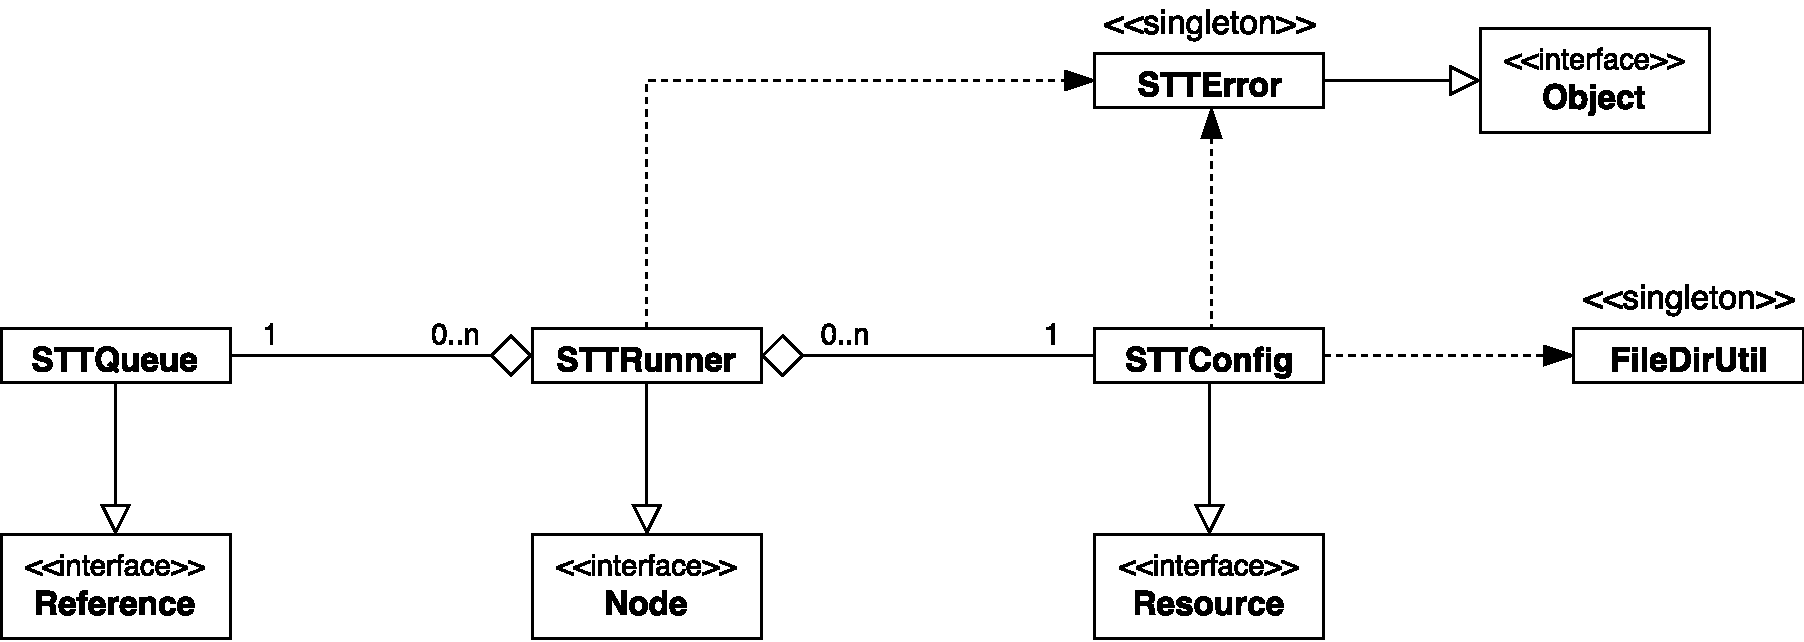
\includegraphics[width=\textwidth]{image/stt-module-simple.pdf}
  \caption{Diagrama de classes simplificado do módulo \textit{Speech to Text}}
  \label{sttModuleClassDiagram}
\end{figure}

Antes de nos aprofundarmos na arquitetura do módulo, algumas observações gerais devem ser feitas:

\begin{itemize}
\item \textit{Godot} não permite que construtores e destrutores possuam argumentos como uma forma de padronizar o instanciamento e liberação de objetos. A restrição aos construtores, no entanto, pode ser contornada através de \textit{setters} para atributos desejados.

\item A \textit{game engine} oferece implementações próprias de alguns tipos e estruturas de dados. Destacamos \texttt{String} para cadeias de caracteres e \texttt{Vector} como um vetor de uso geral, podendo representar uma fila, pilha, etc.

\item O uso de duas classes \textit{singleton} no módulo parece exagero. A justificativa é que \textit{Godot} proíbe a exportação de classes que não podem ser instanciadas (em outras palavras, classes que só possuem métodos estáticos) para uso em \mbox{\textit{GDScript}}. Recomenda-se, portanto, esta outra abordagem para contornar tal limitação \citep{godotStaticClasses}.

\item Quase todas as classes implementadas, exceto \textit{FileDirUtil}, possuem um método especial chamado \texttt{\_bind\_methods()}. Esta função, de nome predefinido por \textit{Godot}, é usada para ligar nomes a constantes ou referências de métodos, permitindo seu uso em \mbox{\textit{GDScript}}. Todas as ligações são guardadas numa grande classe \textit{singleton} denominada \textit{ObjectTypeDB}. A listagem \ref{configBindMethods} exemplifica a adição de uma linha no método \texttt{\_bind\_methods()} de \textit{STTConfig} para ser possível usar o método \texttt{init()} desta mesma classe em \mbox{\textit{GDScript}}.

\begin{lstlisting}[
  language=C++,
  label=configBindMethods,
  caption={Adicionando o método \texttt{init()} de \textit{STTConfig} para uso em \mbox{\textit{GDScript}}}
]
void STTConfig::_bind_methods() {
    ObjectTypeDB::bind_method("init", &STTConfig::init);
}
\end{lstlisting}
\end{itemize}

% ---------------------------------------------------------------------

\subsection{Classe \textit{STTConfig}}
\label{stt-config}

Como o nome sugere, \textit{STTConfig} é uma classe de configuração para a realização do reconhecimento de voz. Por possuir a característica de servir mais como um armazenamento de informação, decidimos fazer a classe herdar de \textit{Resource} (visto na seção \ref{godotResource}).

A figura \ref{stt-config-diagram} apresenta os atributos, métodos e relacionamentos da classe \textit{STTConfig}. O construtor e destrutor foram omitidos por simplicidade. Todos os atributos e métodos estáticos, neste e em futuros diagramas, estarão \underline{sublinhados}.

\begin{figure}[H]
  \centering
  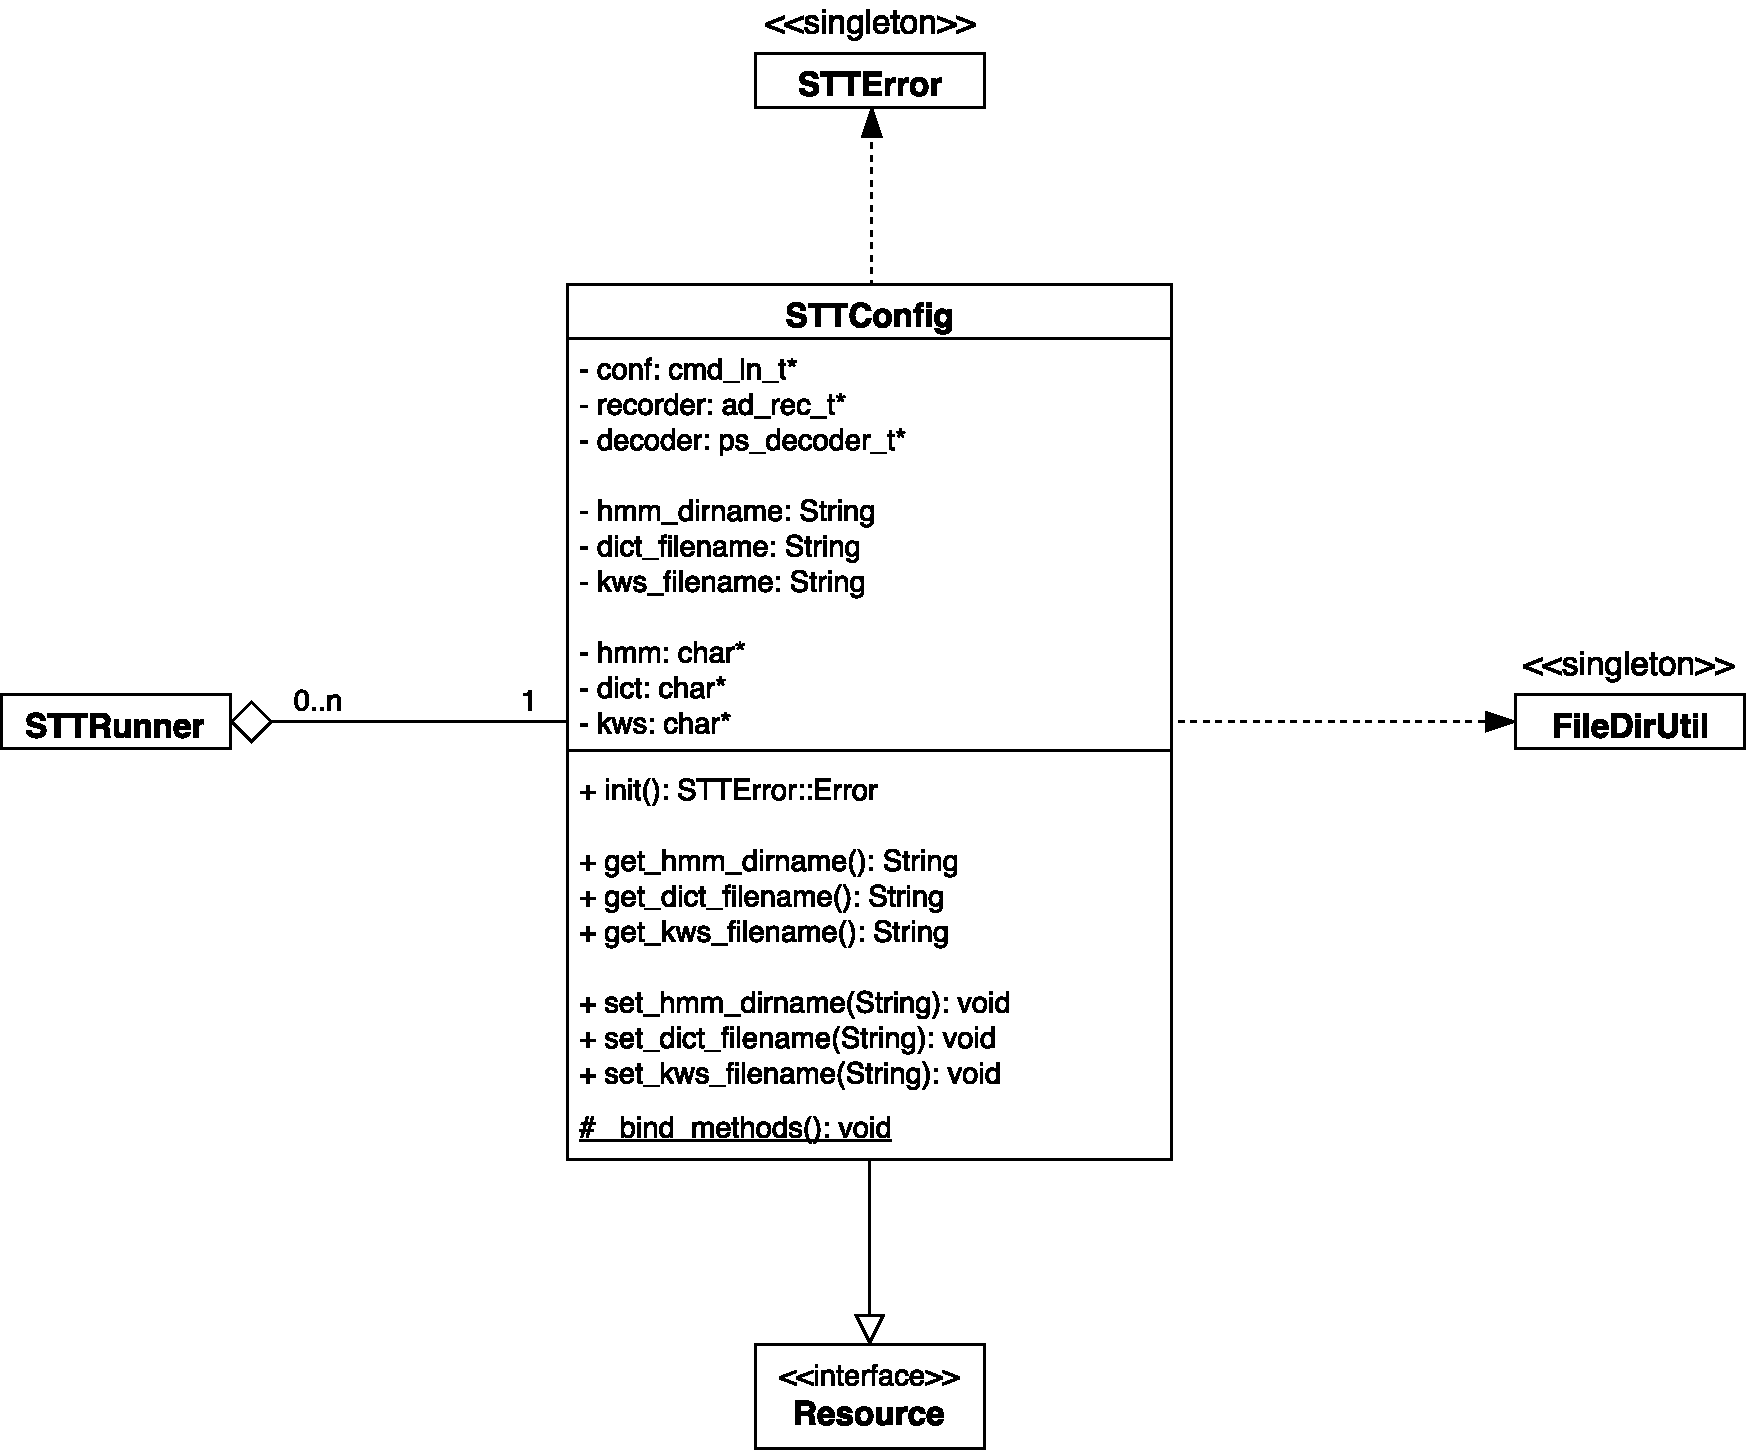
\includegraphics[width=.9\textwidth]{image/stt-config.pdf}
  \caption{Atributos, métodos e relacionamentos da classe \textit{STTConfig}}
  \label{stt-config-diagram}
\end{figure}

\textit{STTConfig} possui duas funcionalidades principais:

\subsubsection{Definir arquivos de configuração}

Nomes de arquivos de configuração são tratados pelos \textit{getters} e \textit{setters} de \texttt{hmm\_dirname}, \texttt{dict\_filename} e \texttt{kws\_filename}, que correspondem, respectivamente, ao diretório do modelo acústico, o arquivo de dicionário e o arquivo de palavras-chaves.

Verifica-se se os nomes passados como argumentos para os \textit{setters} correspondem a arquivos/diretórios existentes. No entanto, infelizmente não há como checar facilmente, em tempo de execução, se o arquivo/diretório possui erros de sintaxe. O diretório do modelo acústico, por exemplo, contém arquivos binários que, a princípio, parecem impossíveis de serem verificados. Optamos, portanto, pela filosofia de ``atirar primeiro, perguntar depois'' ao avisar posteriormente que houve problemas no uso dos arquivos.

Por fim, resta um problema para tratarmos, resultante da distinção entre os sistemas de arquivo de \textit{Godot} (visto na seção \ref{godotFileSystem}) e \textit{Pocketsphinx}. Suponha que o desenvolvedor de um jogo tenha guardado seu arquivo de dicionário, o \texttt{dicionario.dict}, na raiz do projeto. Como referenciar este arquivo? \textit{Godot} utilizaria o caminho \texttt{res://dicionario.dict}, mas \textit{Pocketsphinx} não entende este prefixo, necessitando do caminho absoluto usado no sistema.

Uma solução simples seria converter o caminho com \texttt{res://} para o caminho absoluto do sistema operacional; o método \texttt{globalize\_path} da classe \textit{Globals} de \textit{Godot} faz justamente isso. No entanto, se o jogo estiver no formato de um binário fechado, é impossível referenciar qualquer arquivo dentro dele por meio da plataforma hospedeira.

A solução final implementada envolve usar o outro prefixo definido pela \textit{game engine}, o \textbf{\texttt{user://}}. Copiam-se todos os arquivos e diretórios de configuração para este caminho e usa-se o método \texttt{get\_data\_dir()} da classe \textit{OS} para buscar seu equivalente na plataforma hospedeira. Por precaução, adotou-se a prática de sobrescrever arquivos e diretórios copiados previamente.

\subsubsection{Inicializar variáveis do \textit{Pocketsphinx}}

A inicialização de varíaveis usadas por \textit{Pocketsphinx} é feita através de \texttt{init()}. Os nomes do diretório do modelo acústico, do arquivo de dicionário e do arquivo de palavras-chave precisam ter sido definidos previamente com os apropriados \textit{setters}, ou o método retornará um número de erro.

Deparamo-nos com outro problema de compatibilidade: os nomes dos arquivos são fornecidos com o tipo \texttt{String} adotado por \textit{Godot}. No entanto, \textit{Pocketsphinx} não conhece este tipo, utilizando o \texttt{char *} comumente encontrado em \textit{C} para receber estes mesmos nomes. Felizmente, \texttt{String} possui um método \texttt{c\_str()} para realizar a conversão.

% TODO: Fix reference below

O método \texttt{init()} irá inicializar as variáveis de configuração \texttt{cmd\_ln\_t}, de gravação de voz \texttt{ad\_rec\_t} e o decodificador \texttt{ps\_decoder\_t} (todos vistos na seção \ref{pocketsphinx-structs}). Caso algum problema ocorra, retorna-se um número de erro, pertencente à classe \mbox{\textit{STTError}}, relativo ao problema ocorrido.

A cópia de arquivos para o caminho \textit{user://}, mencionada anteriormente, também ocorre neste método.

% ---------------------------------------------------------------------

\subsection{Classe \textit{STTRunner}}
\label{stt-runner}

\textit{STTRunner} é a classe responsável por realizar o reconhecimento de voz em si. Por claramente implementar uma \textbf{funcionalidade} a ser usada pelo usuário do editor \textit{Godot}, decidiu-se que uma herança de \textit{Node} (visto na seção \ref{godotNode}) seria bastante apropriada.

A figura \ref{stt-runner-diagram} apresenta os atributos, métodos e relacionamentos da classe \textit{STTRunner}. O construtor e destrutor foram omitidos por simplicidade.

\begin{figure}[H]
  \centering
  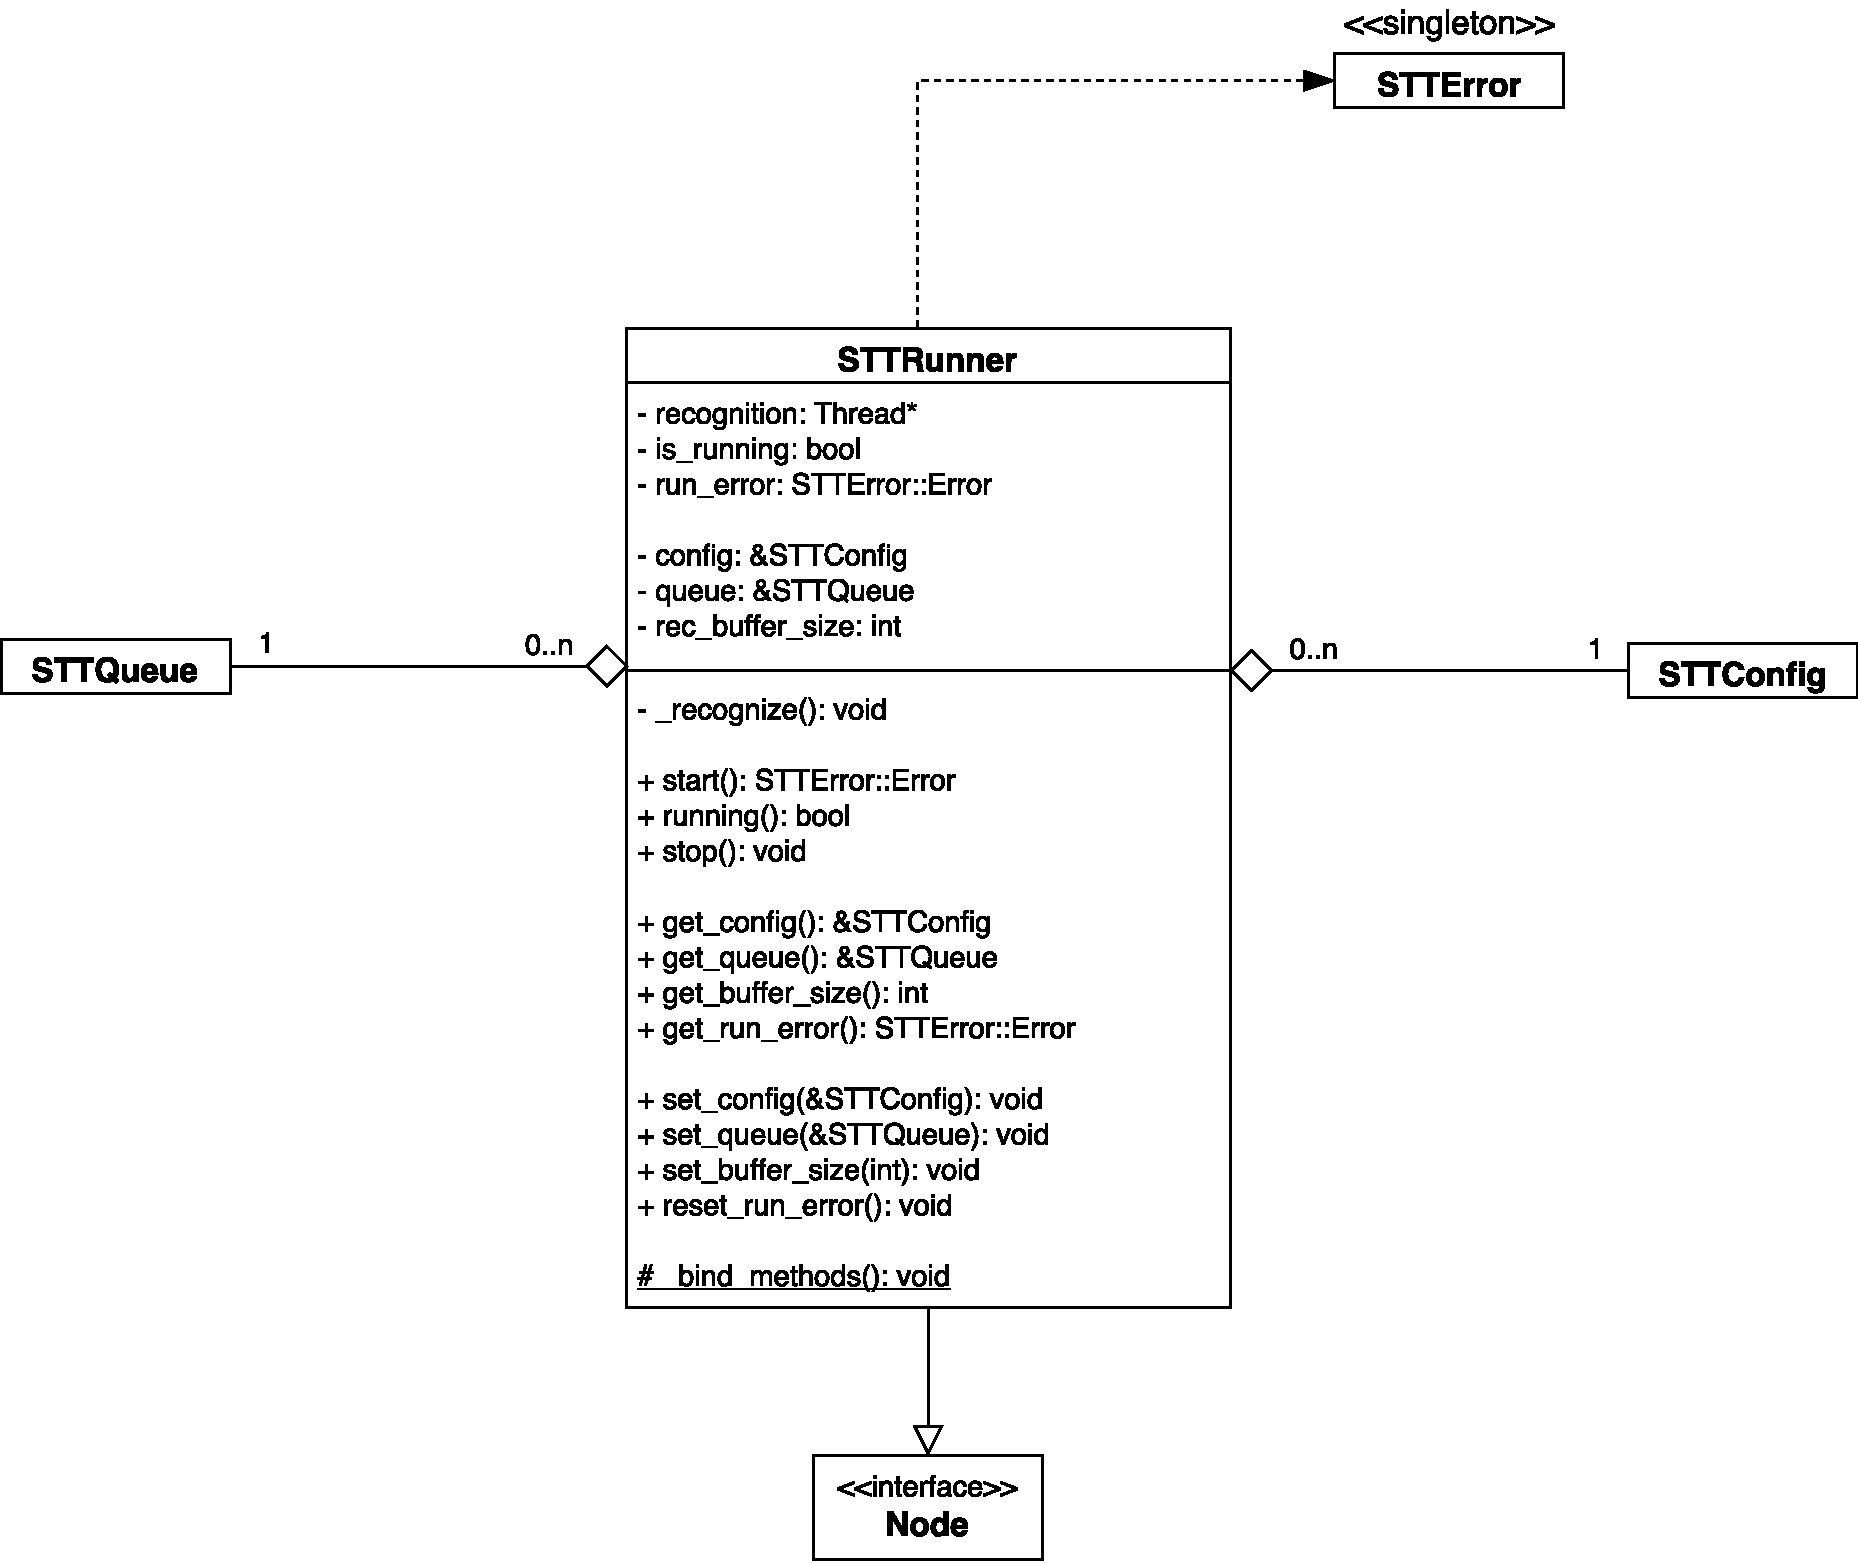
\includegraphics[width=.9\textwidth]{image/stt-runner.pdf}
  \caption{Atributos, métodos e relacionamentos da classe \textit{STTRunner}}
  \label{stt-runner-diagram}
\end{figure}

A classe usa um objeto \textit{STTConfig} para obter as variáveis \textit{Pocketsphinx} necessárias em sua tarefa, e um objeto \textit{STTQueue} para guardar termos (palavras ou pequenas frases) gerados no reconhecimento de voz. Ambos podem ser obtidos e definidos através dos \textit{getters} e \textit{setters} para \texttt{config} e \texttt{queue}.

Comentamos, nos requisitos funcionais (seção \ref{moduleFunctionalRequirements}), que o reconhecimento deveria ocorrer em paralelo com o restante do jogo. O uso de uma \textit{thread} serve bem para tal propósito; \textit{Godot}, inclusive, oferece uma implementação própria dessa estrutura em sua classe \textit{Thread}. Seus dois métodos de maior importância para nós são:

\begin{itemize}
\item \texttt{Thread * create(função, argumento, configurações)}: Cria uma \textit{thread} para executar uma função de assinatura \texttt{func(void *arg)}. O parâmetro \textbf{função} corresponde ao nome da função (neste caso, \texttt{func}) e \textbf{argumento}, a \texttt{arg}. Opcionalmente, podem ser passadas configurações adicionais como um terceiro parâmetro, mas não entraremos em detalhes por não terem sido necessárias. Retorna-se um ponteiro para a instância de \textit{Thread} criada.

\item \texttt{void wait\_to\_finish(thread)}: Recebe um ponteiro para uma instância de \textit{Thread}. Espera a \textit{thread} terminar, finalizando-a com segurança.
\end{itemize}

O método \texttt{start()} cria uma \textit{thread} para realizar o reconhecimento de voz desde que o objeto \textit{STTRunner} já possua instâncias de \textit{STTConfig} e \textit{STTQueue}. Chama-se \texttt{Thread::create()} com um método estático como parâmetro (\texttt{\_thread\_recognize()}, que não aparece na figura \ref{stt-runner-diagram} por agir apenas como um intermédio) e a própria instância como argumento (isto é, \texttt{this}).

A listagem \ref{thread-recognize} mostra a implementação de \texttt{\_thread\_recognize()}, responsável por chamar o método privado \texttt{\_recognize()} da instância passada como argumento. É nesta última função que o laço de reconhecimento de voz ocorre, implementado de forma bastante similar ao que vimos na seção \ref{stt-continuous-algorithm}.

\begin{lstlisting}[
  language=C++,
  label=thread-recognize,
  caption={Método estático \texttt{\_thread\_recognize()} de \textit{STTRunner}}]
void STTRunner::_thread_recognize(void *runner) {
    STTRunner *self = (STTRunner *) runner;
    self->_recognize();
}
\end{lstlisting}

Para controle sobre a \textit{thread}, o usuário do módulo pode verificar sua execução com \texttt{running()} e ordenar sua parada imediata com \texttt{stop()}. Definiu-se que apenas uma \textit{thread} pode existir por instância de \textit{STTRunner}, pois o controle de várias operações em paralelo não traria nenhum benefício ao módulo.

Por fim, oferece-se controle sobre o tamanho do \textit{buffer} de gravação de voz através do \textit{getter} e \textit{setter} de \texttt{buffer\_size}. É importante ressaltar que o uso de um \textit{setter} demanda a parada imediata da \textit{thread} de reconhecimento para evitar possíveis problemas de acesso antes e depois da alteração (\textit{race condition}, ou condição de corrida).

% ---------------------------------------------------------------------

\subsection{Classe \textit{STTQueue}}
\label{stt-queue}

\textit{STTQueue} implementa um \textit{buffer} para guardar palavras geradas no reconhecimento de voz, conforme planejado nos requisitos funcionais (seção \ref{moduleFunctionalRequirements}). Fizemos que com herdasse da classe \textit{Reference} (visto na seção \ref{godotReference}) com o intuito de simplificar seu gerenciamento de memória.

É usado por \textit{STTRunner} para guardar termos do reconhecimento de voz. Ao mesmo tempo, o usuário do módulo pode retirar estes termos do módulo e usá-los no jogo.

A figura \ref{stt-queue-diagram} apresenta os atributos, métodos e relacionamentos da classe \textit{STTQueue}. O construtor e destrutor foram omitidos por simplicidade.

\begin{figure}[H]
  \centering
  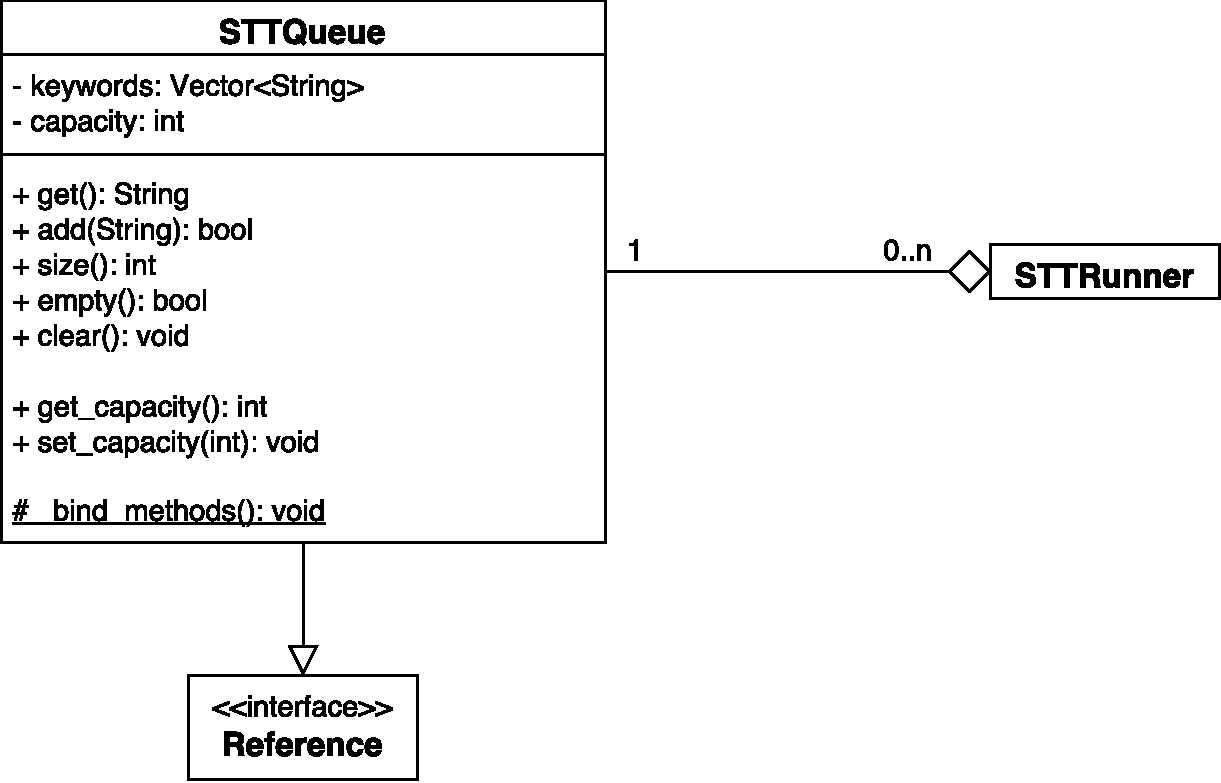
\includegraphics[width=.8\textwidth]{image/stt-queue.pdf}
  \caption{Atributos, métodos e relacionamentos da classe \textit{STTQueue}}
  \label{stt-queue-diagram}
\end{figure}

Conforme o nome sugere, o tipo abstrato de dados usado para o \textit{buffer} da \textit{STTQueue} é uma \textbf{fila}. \textit{Godot} implementa esta estrutura, com diversas funcionalidade a mais, em sua classe \textit{Vector}. Como muitas de seus métodos seriam desnecessários (não é necessário, por exemplo, que o usuário possa ordenar a fila de reconhecimento de voz), \textit{STTQueue} age como um intermédio do que pode e não pode ser feito em \textit{Vector}.

Os principais métodos de \textit{STTQueue} estão resumidos na tabela \ref{stt-queue-main-methods}.

\begin{table}[H]
\centering

\begin{tabular}{|c|l|}
\hline
\textbf{Método}  & \thead{\textbf{Descrição}}                          \\ \hline
\texttt{get()}   & Retira e retorna a primeira \texttt{String} da fila \\ \hline
\texttt{add()}   & Adiciona uma \texttt{String} no final da fila       \\ \hline
\texttt{size()}  & Retorna o número de elementos atualmente na fila    \\ \hline
\texttt{empty()} & Retorna \texttt{true} se a fila estiver vazia       \\ \hline
\texttt{clear()} & Esvazia a fila, removendo todos os seus elementos   \\ \hline
\end{tabular}

\caption{Principais métodos de \textit{STTQueue}}
\label{stt-queue-main-methods}
\end{table}

O leitor pode se perguntar se não ocorre condição de corrida no acesso à fila: há risco de se perder algum dado quando \textit{STTRunner} realiza um \texttt{add()} ao mesmo tempo em que o usuário utiliza \texttt{get()}, por exemplo? Felizmente, a implementação de \texttt{Vector} é \textit{thread-safe}, garantindo que esses problemas não ocorram.

Uma decisão deveria ser tomada quanto a um caso particular de \texttt{get()}: o que fazer quando o método fosse chamado com uma fila vazia? Nesta situação, decidiu-se retornar uma \texttt{String} vazia (\texttt{``''}) e simultaneamente imprimir uma mensagem de \textit{warning} devido ao uso impróprio. Recomenda-se, portanto, verificar o tamanho da fila com \texttt{empty()} antes do uso de \texttt{get()}.

Além dos métodos da tabela \ref{stt-queue-main-methods}, há mais dois que foram criados para definir um limite superior para o número de elementos na fila. Este valor pode ser lido e alterado por \texttt{get\_capacity()} e \texttt{set\_capacity()}, respectivamente. O usuário, teoricamente, não deveria permitir um acúmulo muito grande de palavras na fila, mas se tal caso ocorrer, ao menos o consumo de memória fica controlado.

% ---------------------------------------------------------------------

\subsection{Classe \textit{STTError}}

\textit{STTError} define constantes numéricas para possíveis erros que podem ocorrer no módulo (mais especificamente, em \textit{STTConfig} e \textit{STTRunner}). A utilidade da classe, portanto, está em ajudar o usuário a entender melhor a causa de um erro que possa vir a ocorrer no módulo. Por ser um \textit{singleton} mas ter seu uso necessário no editor \textit{Godot} (através de \mbox{\textit{GDScript}}), decidiu-se fazer a classse herdar de \textit{Object} (visto na seção \ref{godotObject}).

A figura \ref{stt-error-diagram} apresenta os atributos, métodos e relacionamentos da classe \textit{STTError}. O construtor e destrutor foram omitidos por simplicidade.

\begin{figure}[H]
  \centering
  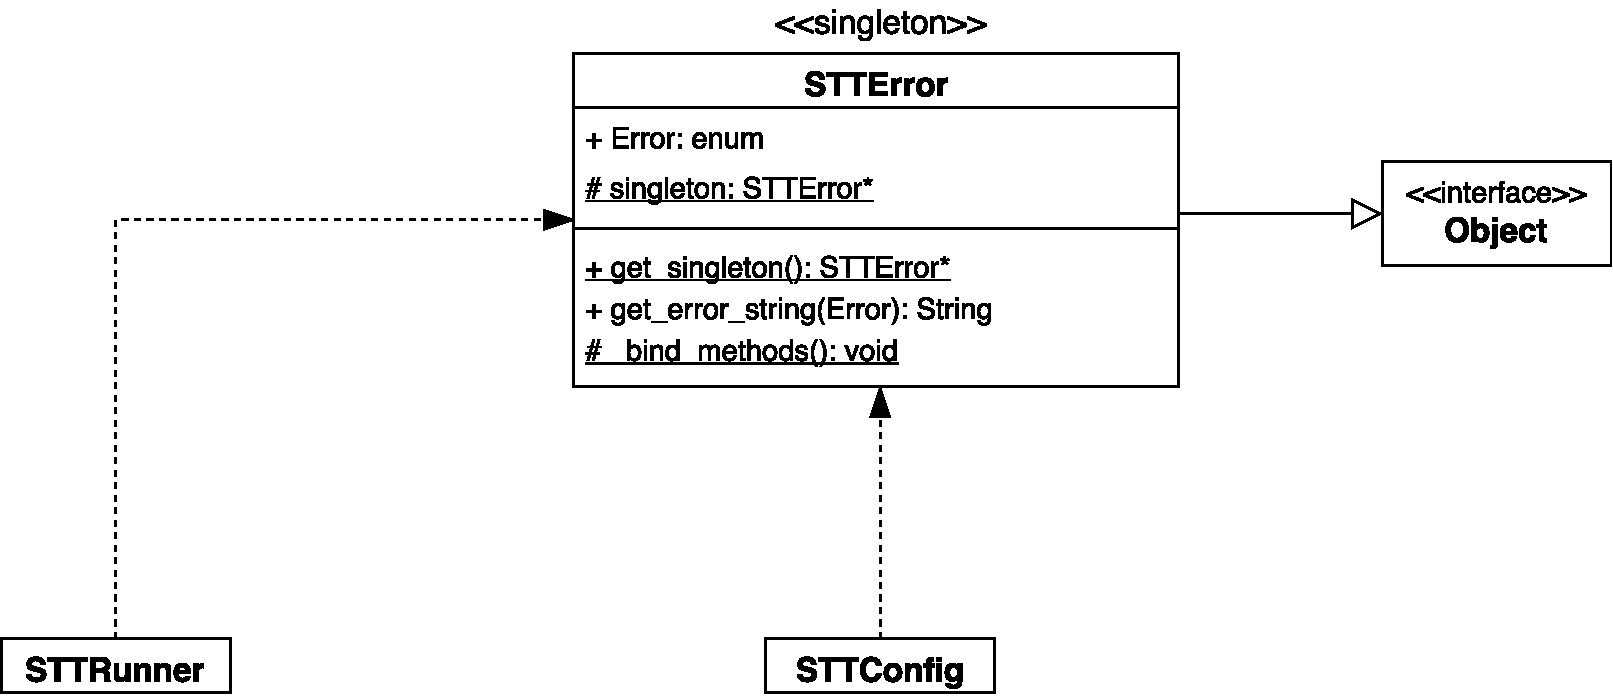
\includegraphics[width=.9\textwidth]{image/stt-error.pdf}
  \caption{Atributos, métodos e relacionamentos da classe \textit{STTError}}
  \label{stt-error-diagram}
\end{figure}

Alguns métodos de \textit{STTConfig} e \textit{STTRunner} retornam um número definido pelo \texttt{enum Error}. Uma \texttt{String} contendo a interpretação deste valor pode ser obtida chamando-se o método \texttt{get\_error\_string()} da classe.

A tabela \ref{stt-error-enum} contém os valores definidos no \texttt{enum Error}, bem como suas respectivas interpretações.

\begin{table}[H]
\centering

\begin{tabularx}{\linewidth}{|l|X|}
\hline
\thead{\textbf{Erro}} & \thead{\textbf{Interpretação}} \\ \hline
\texttt{OK} & Nenhum erro ocorreu \\ \hline
\texttt{UNDEF\_FILES\_ERR} & Um ou mais nomes de arquivos/diretórios de configuração não foram definidos \\ \hline
\texttt{UNDEF\_CONFIG\_ERR} & Um objeto \texttt{STTConfig} não foi definido \\ \hline
\texttt{UNDER\_QUEUE\_ERR} & Um objeto \texttt{STTQueue} não foi definido \\ \hline
\texttt{USER\_DIR\_MAKE\_ERR} & Erro ao criar o diretório STT em \texttt{user://} \\ \hline
\texttt{USER\_DIR\_COPY\_ERR} & Erro ao copiar arquivos de configuração para \texttt{user://} \\ \hline
\texttt{MULTIBYTE\_STR\_ERR} & Erro ao converter o nome do arquivo para uma sequência de vários bytes \\ \hline
\texttt{MEM\_ALLOC\_ERR} & Não há memória disponível para alocação \\ \hline
\texttt{CONFIG\_CREATE\_ERR} & Erro ao criar a variável de configuração de \textit{Pocketsphinx} \\ \hline
\texttt{REC\_CREATE\_ERR} & Erro ao se conectar o aparelho de áudio (microfone) \\ \hline
\texttt{DECODER\_CREATE\_ERR} & Erro ao criar a variável de decodificação de \textit{Sphinxbase} \\ \hline
\texttt{REC\_START\_ERR} & Erro ao começar a gravar a voz do usuário \\ \hline
\texttt{REC\_STOP\_ERR} & Não foi possível parar a gravação da voz do usuário \\ \hline
\texttt{UTT\_START\_ERR} & Erro ao iniciar a captura de \textit{utterance} durante o reconhecimento de voz \\ \hline
\texttt{UTT\_RESTART\_ERR} & Erro ao reiniciar a captura de \textit{utterance} durante o reconhecimento de voz \\ \hline
\texttt{AUDIO\_READ\_ERR} & Erro ao ler dados da gravação de áudio \\ \hline
\end{tabularx}

\caption{Valores de erro definidos em \texttt{enum Error} e suas interpretações}
\label{stt-error-enum}
\end{table}

% ---------------------------------------------------------------------

\subsection{Classe \textit{FileDirUtil}}

\textit{FileDirUtil} é uma classe auxiliar, não possuindo relação alguma com reconhecimento de voz. Como o nome sugere, ela possui métodos para manipular arquivos e diretórios.

A figura \ref{file-dir-util-diagram} apresenta os métodos e relacionamento da classe \textit{FileDirUtil}. O construtor e destrutor foram omitidos por simplicidade.

\begin{figure}[H]
  \centering
  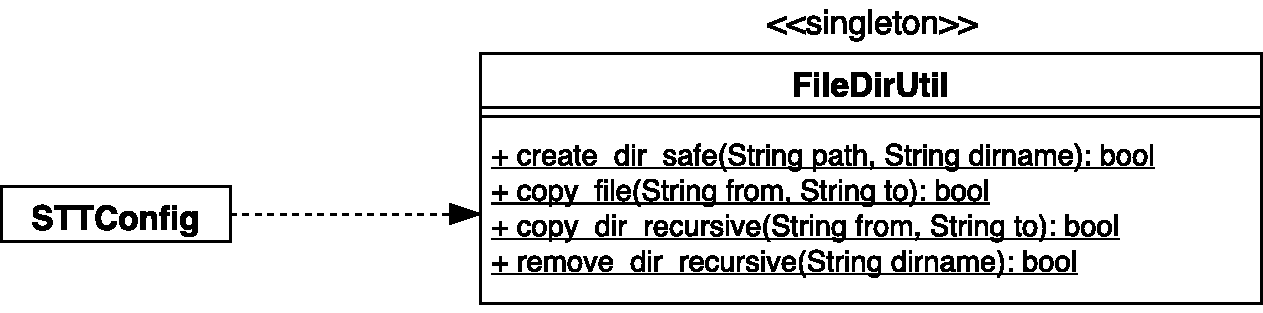
\includegraphics[width=.75\textwidth]{image/file-dir-util.pdf}
  \caption{Atributos, métodos e relacionamentos da classe \textit{FileDirUtil}}
  \label{file-dir-util-diagram}
\end{figure}

As ferramentas oferecidas por \textit{Godot} para gerenciamento de arquivos e diretórios são bem simples, limitando-se ao seguinte: criação de arquivos/diretórios, escrita/leitura/cópia de arquivos, remoção de arquivos individuais e diretórios vazios.

Vimos que \textit{STTConfig} necessita copiar os arquivos de configuração para \texttt{user://}. \textit{FileDirUtil} meramente combina os métodos já implementados pela \textit{game engine} para realizar operações como cópia e remoção recursiva de diretórios.

% ---------------------------------------------------------------------

\section{Arquivos e \textit{scripts} de configuração}

Com a implementação feita, faltam apenas alguns arquivos e \textit{scripts} que informam a existência das classes a \textit{Godot}, bem como a forma de compilar o código fonte do módulo.

% ---------------------------------------------------------------------

\subsection{Registro de tipos}

\textit{Godot} exige dois arquivos adicionais, \texttt{register\_types.h} e \texttt{register\_types.cpp}, para controlar quais classes do módulo poderão ser usadas em \mbox{\textit{GDScript}}. Duas funções obrigatoriamente devem ser implementadas, com o nome do módulo no meio de seu nome:

\subsubsection{\texttt{register\_speech\_to\_text\_types()}}

Serve para registrar classes no banco de dados \textit{ObjectTypeDB}. A implementação desta função no módulo \textit{Speech to Text} é apresentada na listagem \ref{register-types}.

\begin{lstlisting}[
  language=C++,
  label=register-types,
  caption={Implementação de \texttt{register\_speech\_to\_text\_types()}}]
static STTError *stt_error = NULL;

void register_speech_to_text_types() {
    ObjectTypeDB::register_type<STTConfig>();
    ObjectTypeDB::register_type<STTQueue>();
    ObjectTypeDB::register_type<STTRunner>();
    ObjectTypeDB::register_virtual_type<STTError>();

    stt_error = memnew(STTError);
    Globals::get_singleton()->add_singleton(
        Globals::Singleton("STTError", STTError::get_singleton()));
}
\end{lstlisting}

O método \texttt{register\_type} de \textit{ObjectTypeDB} faz o registro da classe. Há um caso especial em \textit{STTError}, que usa \texttt{register\_virtual\_type} para não ser instanciável. Por fim, como esta mesma classe é um \textit{singleton}, aproveitamos para criar sua única instância com \texttt{memnew()} (o equivalente de \texttt{new} para \textit{Godot}) e guardar umas referência junto a outros \textit{singletons} em \textit{Globals}.

\subsubsection{\texttt{unregister\_speech\_to\_text\_types()}}

Esta função é chamada após o jogo ser finalizado (fechado). Tipicamente é usada para desalocar memória e/ou realizar tarefas de término no módulo. A implementação desta função no módulo \textit{Speech to Text} é apresentada na listagem \ref{unregister-types}.

\begin{lstlisting}[
  language=C++,
  label=unregister-types,
  caption={Implementação de \texttt{unregister\_speech\_to\_text\_types()}}]
void unregister_speech_to_text_types() {
    if (stt_error) memdelete(stt_error);

    // Remove all STT data in user://
    String user_dirname = "user://" + String(STT_USER_DIRNAME);
    if (DirAccess::exists(user_dirname))
        FileDirUtil::remove_dir_recursive(user_dirname);
}
\end{lstlisting}

Em nosso caso, basta liberar o \textit{singleton} de \textit{STTError} alocado previamente; note que \texttt{memdelete} é o equivalente de \texttt{delete} em \textit{Godot}. Também removemos todos os arquivos de configuração copiados para \texttt{user://} pela classe \textit{STTConfig}.

% ---------------------------------------------------------------------

\subsection{\texttt{SCsub}}

Já vimos que \textit{SCons} é a ferramenta usada na compilação de \textit{Godot} (seção \ref{scons}), utilizando-se de \textit{scripts} escritos em \textit{Python} para definir seu comportamento. Com módulos não é diferente, necessitando-se de um \textit{script} de nome \texttt{SCsub}.

A implementação deste script envolve listar quais os arquivos a serem compilados e quais \textit{flags} o compilador deve usar.

Percebemos que uma compilação em \textit{Windows} era possível devido à facilidade da ferramenta; bastou adicionar um arquivo próprio de \textit{Pocketsphinx} (\texttt{ad\_win32.c}) que opera especificamente sobre este sistema operacional.

% ---------------------------------------------------------------------

\subsection{\texttt{config.py}}

A última configuração necessária é dada pelo \textit{script} em \textit{Python} \texttt{config.py}. Ele possui duas funções com propósitos diferentes:

\subsubsection{\texttt{can\_build(platform)}}

Esta função recebe o nome da plataforma em que \textit{Godot} está sendo compilado. Retorna-se \texttt{True} se o módulo pode ser compilado nela ou \texttt{False} caso contrário.

A listagem \ref{can-build} apresenta a implementação da função.

\begin{lstlisting}[
  language=Python,
  label=can-build,
  caption={Função \texttt{can\_build()} em \texttt{config.py}}]
import os

def can_build(platform):
   if platform == "x11":
      has_pulse = os.system("pkg-config --exists libpulse-simple") == 0
      has_alsa = os.system("pkg-config --exists alsa") == 0
      return has_pulse or has_alsa
   elif platform == "windows":
      return True
   else:
      return False
\end{lstlisting}

Em nosso caso, \textit{Speech to Text} deve verificar se a plataforma \textit{Unix} (referida como \textit{x11}) possui sistema de som \textit{PulseAudio} \citep{pulseaudio} ou \textit{ALSA} \citep{alsa}, pois ambos são compatíveis tanto com \textit{Godot} quanto com \textit{Pocketsphinx}. Sistemas \textit{Windows} são, teoricamente, sempre compatíveis devido a um arquivo de \textit{Pocketsphinx} que trata seu sistema de som. Outros sistemas operacionais não foram testados, então preferiu-se retornar \texttt{False}.

\subsubsection{\texttt{configure(env)}}

Recebe um objeto caracterizando o ambiente de compilação, podendo realizar ajustes nele independentemente dos arquivos existentes no módulo.

Nenhuma mudança foi necessária em \textit{Speech to Text}, o que levou esta função a ficar sem conteúdo (listagem \ref{configure}).

\begin{lstlisting}[
  language=Python,
  label=configure,
  caption={Função \texttt{configure()} em \texttt{config.py}}]
def configure(env):
   pass
\end{lstlisting}

% ---------------------------------------------------------------------

\section{Divulgação}
\label{modulePublishing}

Todo o código fonte do módulo \textit{Speech to Text} encontra-se em um repositório no GitHub do autor \citep{sttModuleGitHub}, juntamente com instruções para compilação. Um tutorial para seu uso no editor, baseado no formato usado na documentação da própria \textit{game engine}, encontra-se no repositório \citep{sttModuleTutorial}. Também foram disponibilizados binários dos editores \textit{Godot} e \textit{templates de exportação}, ambos compilados previamente com o módulo, para \textit{Windows} e \textit{Unix} \citep{sttModuleDownload}.

A compilação com o módulo é bastante simples: basta baixar o diretório de \textit{Speech to Text} que deve ser inserido em \texttt{modules/} e recompilar \textit{Godot}, seguindo os mesmos passos apresentados na seção \ref{godotCompile}.

\textit{Speech to Text} foi divulgado em dois fóruns de \textit{Godot}, onde obteve algumas poucas aprovações:

\begin{itemize}
\item \textbf{Godot Engine Q\&A} \citep{sttModuleGodotQA}: O site oficial de \textit{Godot} disponibiliza uma seção para perguntas e respostas, onde existe uma subseção para publicação de projetos.

\item \textbf{Godot Developers} \citep{sttModuleGodotDevelopers}: Embora seja mais voltado para jogos produzidos na \textit{game engine}, este fórum possui uma seção para compartilhamento de recursos e ferramentas.
\end{itemize}

\chapter{Jogo \textit{Color Clutter}}
\label{cap:color-clutter}

Dado que o módulo \textit{Speech to Text} está agora pronto, desenvolveremos um pequeno jogo com ele através do editor \textit{Godot} para demonstrar seu uso e analisar a qualidade do reconhecimento de voz na prática.

Ao longo deste capítulo, relatamos os passos realizados na criação do jogo \textit{Color Clutter}. Para melhor aproveitamento, o leitor precisará do editor \textit{Godot}, na versão 2.1.4, com o módulo instalado. Mencionamos, na seção \ref{modulePublishing}, alguns \textit{links} para baixar uma versão já pronta e para obter instruções de como compilar \textit{Speech to Text} com a \textit{game engine}.

% ---------------------------------------------------------------------

\section{Uso do editor \textit{Godot}}

Antes de começarmos o desenvolvimento do jogo, iremos descrever alguns elementos da interface do editor \textit{Godot} para melhor familiarizar o leitor com esta ferramenta.

% ---------------------------------------------------------------------

\subsection{Gerenciamento de projetos}

Ao executar o editor \textit{Godot}, o leitor é confrontado com a tela apresentada na figura \ref{editor-project-select}, na qual pode gerenciar seus projetos (jogos).

\begin{figure}[H]
  \centering
  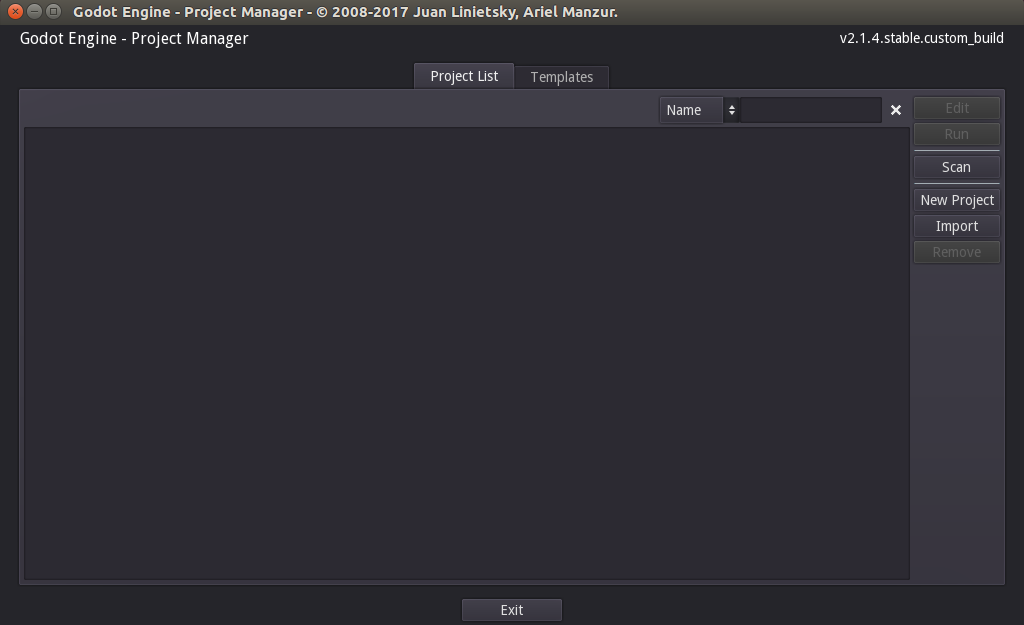
\includegraphics[width=.85\textwidth]{image/editor-project-select}
  \caption{Gerenciamento de projetos no editor \textit{Godot}}
  \label{editor-project-select}
\end{figure}

Projetos são listados na aba \textit{Project List}, onde podem ser abertos para edição ou removidos. Também é possível criar um novo jogo ou a importar um já existente. A criação de um projeto, por exemplo, é feita pelo botão \textit{New Project} e requer a especificação do caminho na qual será criado (\textit{Project Path}) e seu nome (\textit{Project Name}). Já a importação exige que o usuário escolha um caminho que contenha o arquivo \texttt{engine.cfg}, responsável por definir o diretório raiz do jogo.

Na figura \ref{editor-project-create}, exemplificamos a criação do projeto \textbf{teste} no diretório \texttt{\textasciitilde/Desktop/teste}. Ao clicar no botão \textit{Create}, o projeto é criado e o usuário é automaticamente encaminhado para a tela de edição de \textbf{teste}.

\begin{figure}[H]
  \centering
  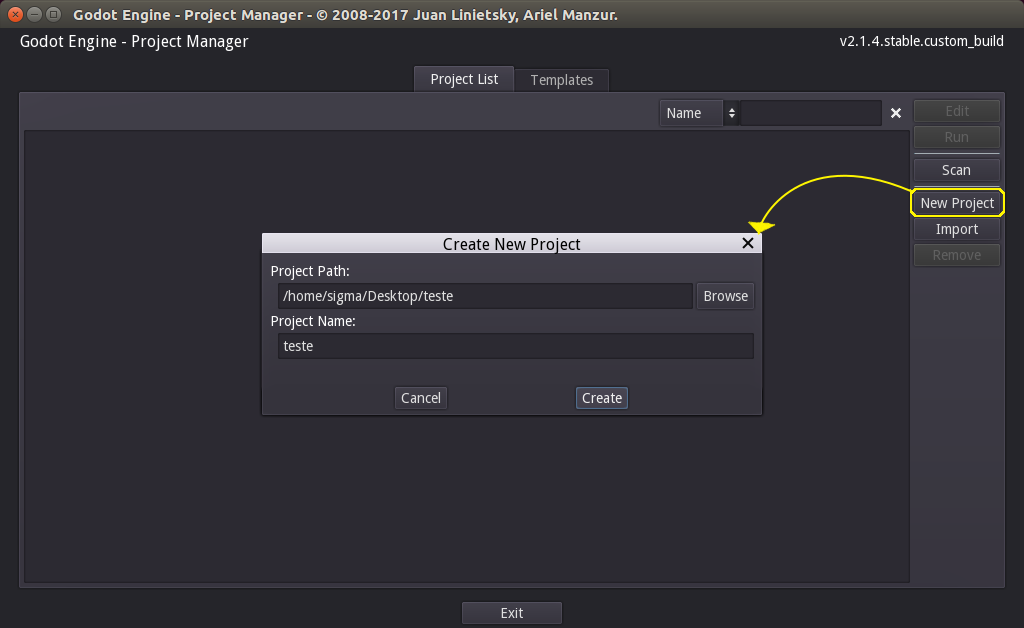
\includegraphics[width=.85\textwidth]{image/editor-project-create-edit}
  \caption{Criação do projeto \textbf{teste} no editor \textit{Godot}}
  \label{editor-project-create}
\end{figure}

% ---------------------------------------------------------------------

\subsection{Interface de edição de um projeto}

A criação de um novo projeto leva o usuário ao editor do mesmo. Continuando com nosso exemplo \textbf{teste}, sua tela de edição é apresentada na figura \ref{in-game-editor}.

\begin{figure}[H]
  \centering
  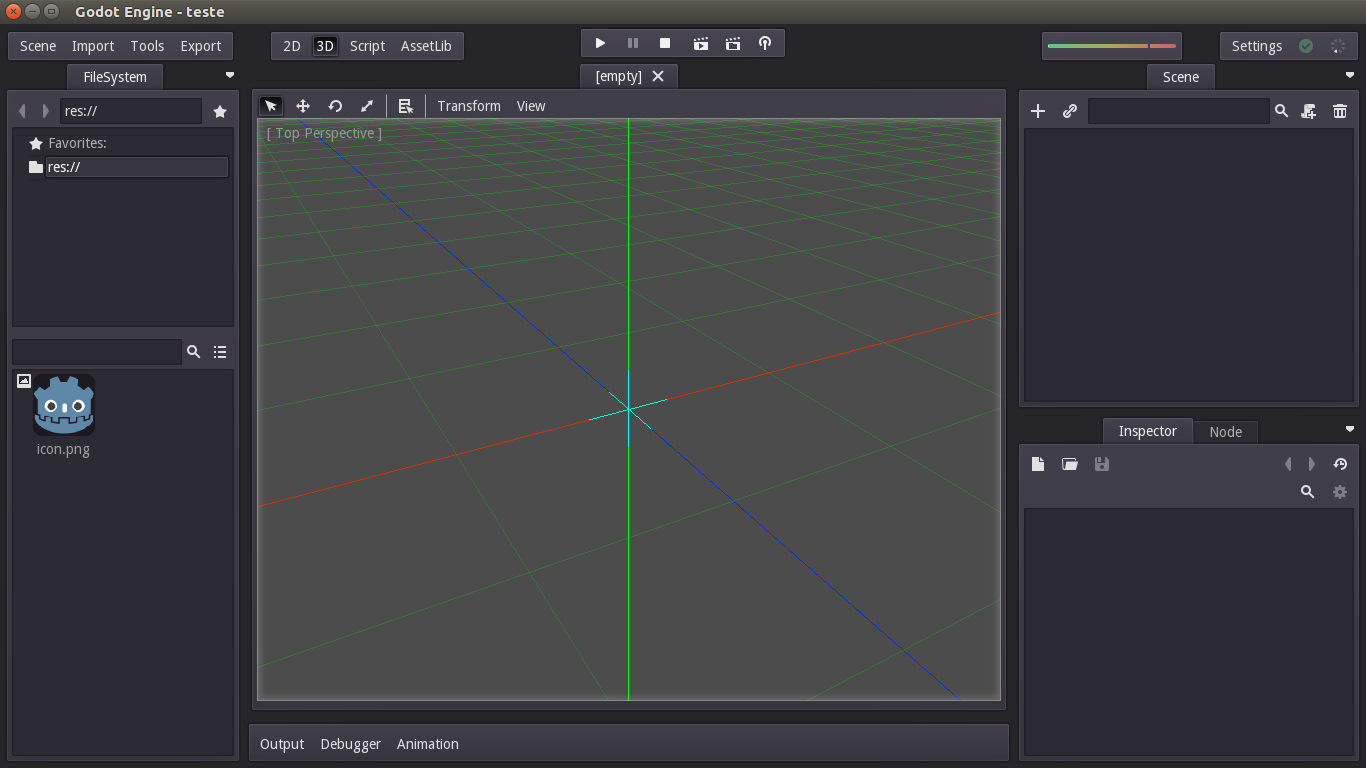
\includegraphics[width=.9\textwidth]{image/in-game-editor}
  \caption{Editor de um projeto \textit{Godot} (neste caso, \textbf{teste})}
  \label{in-game-editor}
\end{figure}

Uma explicação detalhada de todas as funcionalidades do editor fugiria do tema deste trabalho. Iremos, portanto, nos atentar às ferramentas principais, apresentadas a seguir.

% ---------------------------------------------------------------------

\subsection{Uso de \textit{nodes} e \textit{scenes}}

No canto superior direito do editor (conforme a figura \ref{in-game-editor}, a \textit{scene} (explicada na seção \ref{godotScene}) atual do projeto é indicada na aba de mesmo nome. É neste espaço que a hierarquia de \textit{nodes} (definidos na seção \ref{godotNode} pertencentes a esta cena é apresentada.

A criação de um \textit{node} para a cena é feita através do símbolo \textbf{\texttt{+}} desta aba, que leva o usuário a uma lista de nós existentes (figura \ref{editor-node}). Por curiosidade, recomenda-se que o leitor procure o nó \textbf{\textit{STTRunner}} (descrito na seção \ref{stt-runner}), fornecido pelo módulo \textit{Speech to Text}.

\begin{figure}[H]
  \centering
  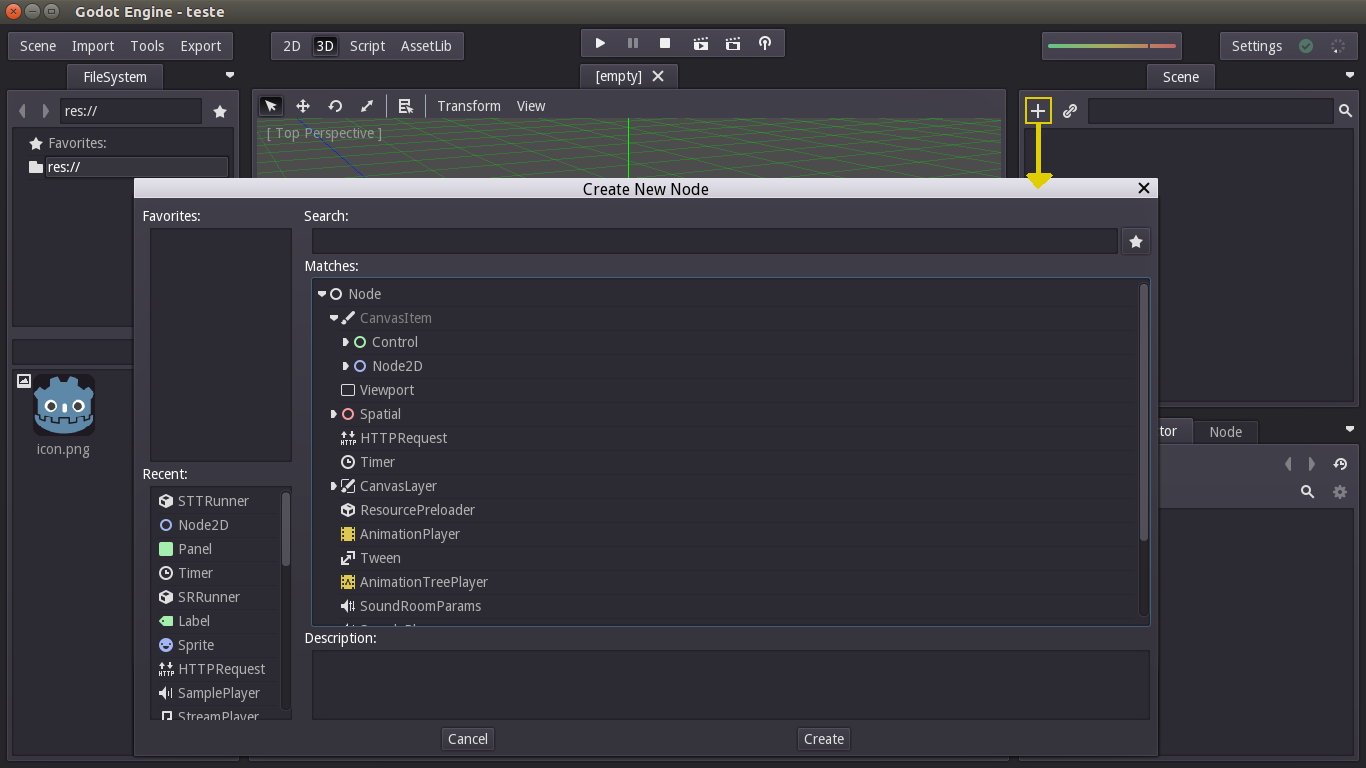
\includegraphics[width=.9\textwidth]{image/editor-node-edit}
  \caption{Lista de \textit{nodes} disponíveis no editor do projeto}
  \label{editor-node}
\end{figure}

Como exemplo, escolheremos, nesta lista, o \textit{node} \textbf{\textit{Label}} para representar um texto. A aba \textit{Scene} mostrará que foi adicionada à cena. Além disso, se selecionarmos este nó, a aba debaixo, \textit{Inspector}, indicará quais as suas propriedades editáveis, enquanto a janela central do editor mostrará seu posicionamento em relação a outros elementos do jogo (figura \ref{editor-label}).

\begin{figure}[H]
  \centering
  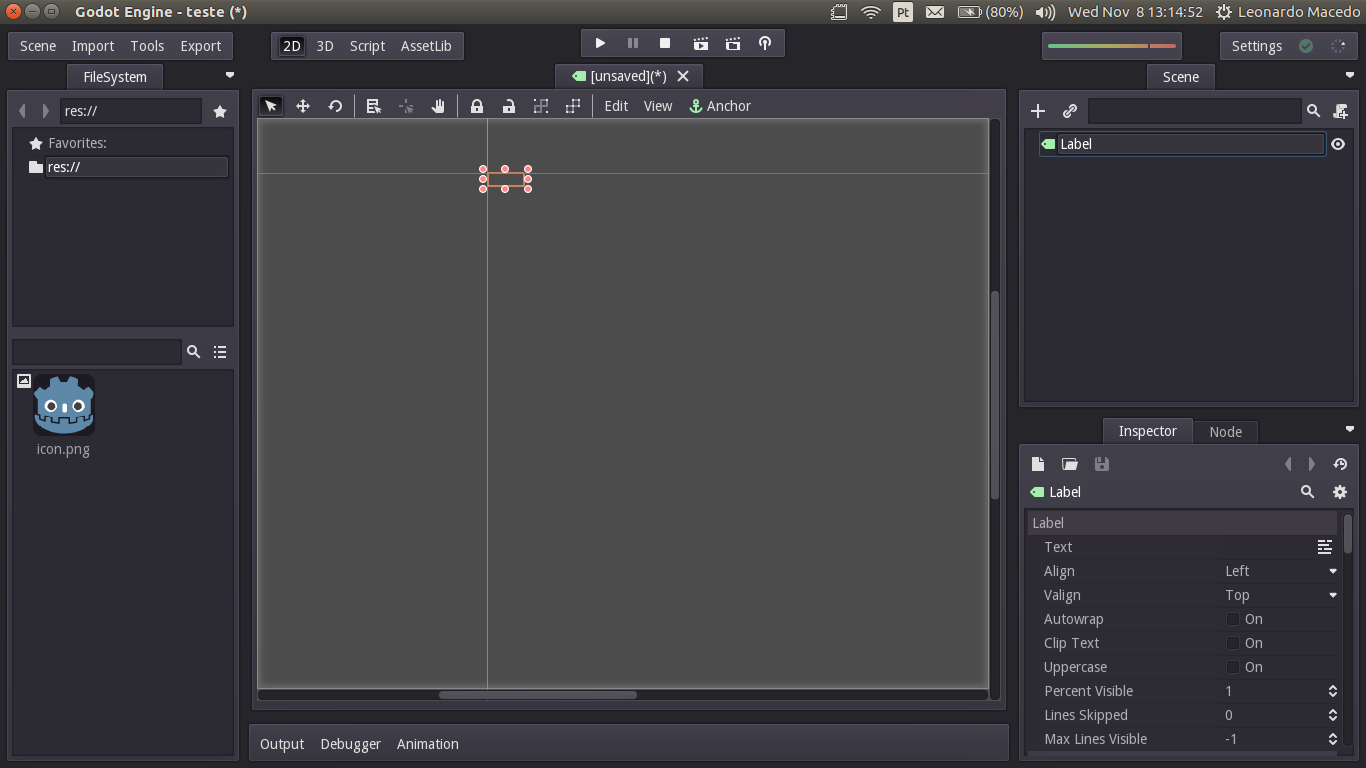
\includegraphics[width=.9\textwidth]{image/editor-label}
  \caption{Edição do \textit{node} \textbf{\textit{Label}}; note suas propriedadas na aba \textit{Inspector} (canto inferior direito)}
  \label{editor-label}
\end{figure}

Suponha que desejamos executar o jogo com apenas o nó \textit{Label}, com ele apresentando o texto \textit{``Hello World!''}. Para tanto, seguiremos os seguintes passos, ilustrados melhor pela figura \ref{editor-run-scene-edit}.

\begin{figure}[H]
  \centering
  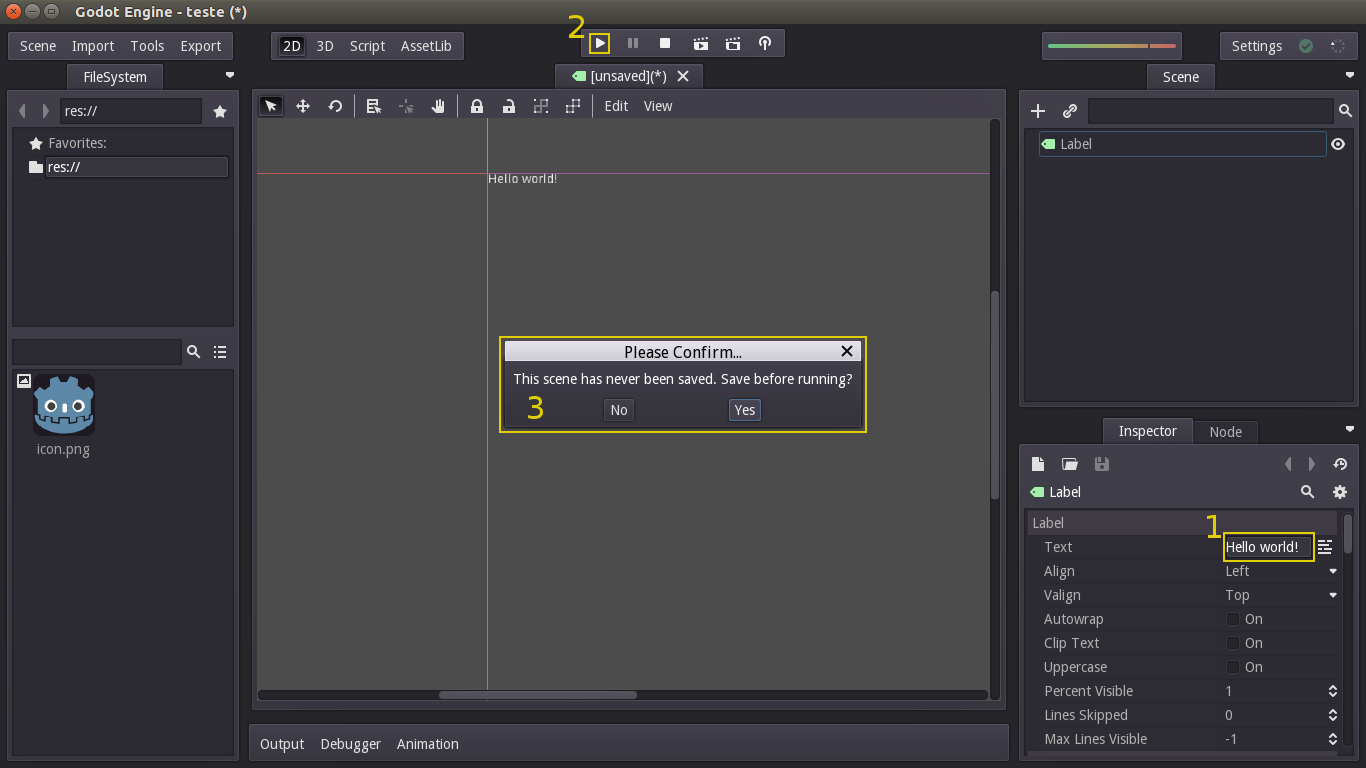
\includegraphics[width=.9\textwidth]{image/editor-run-scene-edit}
  \caption{Passos para execução da \textit{scene} contendo um \textit{Label} escrito \textit{``Hello World!''}}
  \label{editor-run-scene-edit}
\end{figure}

\begin{itemize}
\item Alterar o texto do \textit{Label} para \textit{``Hello World!''}. Isto é facilmente feito pela propriedade \textbf{\textit{Text}} na aba \textit{Inspector} (\textbf{1} na figura \ref{editor-run-scene-edit}).

\item Salvar a \textit{scene} atual. Uma forma de fazer isso para depois executar o jogo é clicar no botão \textit{Play the project} (triângulo no centro superior do editor; vide \textbf{2} na figura \ref{editor-run-scene-edit}). O editor apresentará uma janela para salvar a cena (\textbf{3} na figura \ref{editor-run-scene-edit}) como um arquivo cujo formato padrão é \texttt{.tscn}.

\item Se \textit{Play the project} foi usado para salvar a cena, imediatamente outra janela será exibida, solicitando a escolha da \textit{scene} a ser usada quando o jogo é iniciado. Basta escolher o arquivo \texttt{.tscn} que foi salvo no passo anterior.
\end{itemize}

O resultado, apresentado na figura \ref{editor-hello-world}, será a abertura de uma nova janela para a execução do jogo. Note o texto \textit{``Hello World!''} em seu canto superior esquerdo.

\begin{figure}[H]
  \centering
  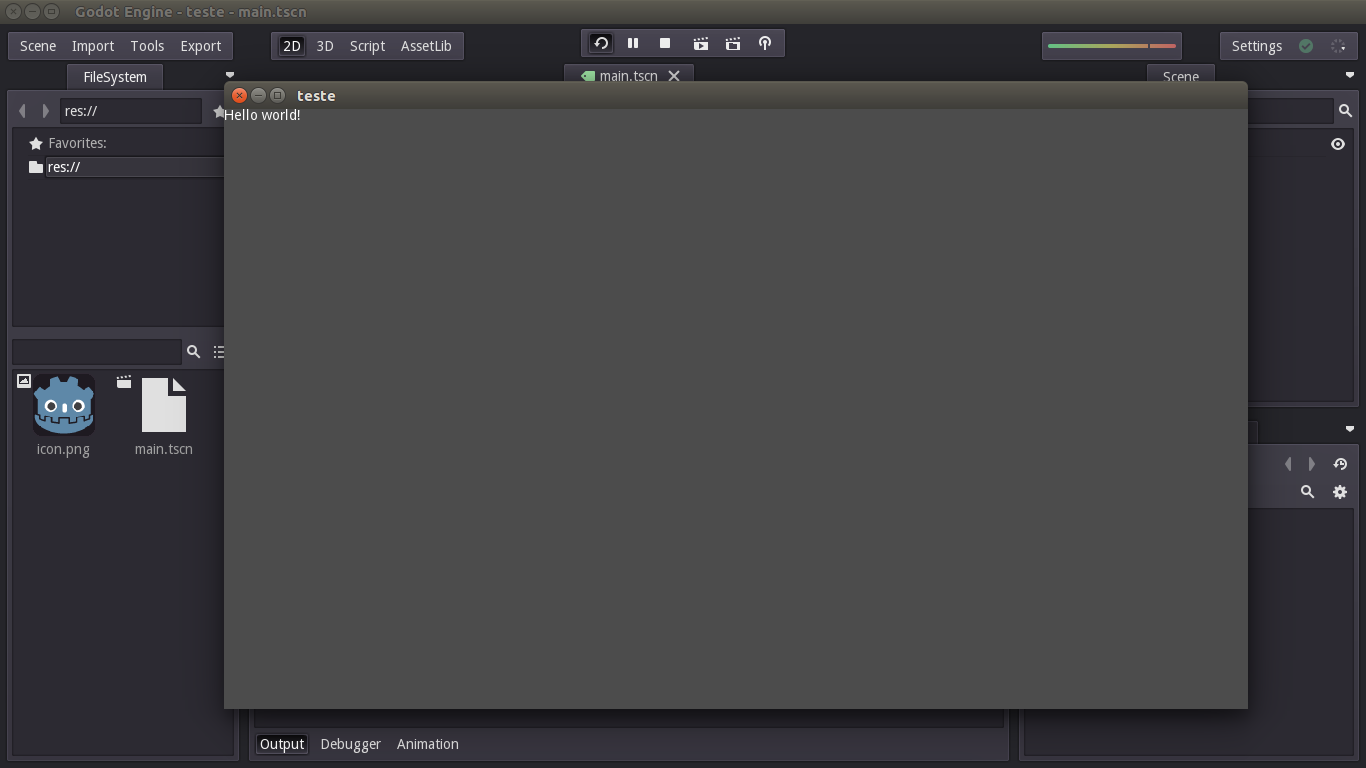
\includegraphics[width=.9\textwidth]{image/editor-hello-world}
  \caption{Execução da \textit{scene} contendo um \textit{Label} de texto \textit{``Hello world!''}}
  \label{editor-hello-world}
\end{figure}

% ---------------------------------------------------------------------

\subsection{Uso de \textit{GDScript}}

A linguagem \textit{GDScript} (introduzida na seção \ref{godotLanguages}) é usada para escrever trechos de código que definem o comportamento de \textit{nodes} \citep{godotScripting}.

Para adicionar um \textit{script} a um nó, basta clicar em seu nome, na aba \textit{Scene}, com o botão direito e escolher \textbf{\textit{Add Script}} (figura \ref{editor-attach-script}). Uma janela irá surgir, onde é necessário preencher apenas o campo \textit{Path} para definir o nome do \textit{script} (figura \ref{editor-script-window}).

\begin{figure}[H]
  \centering

  \begin{minipage}{.5\textwidth}
    \centering
    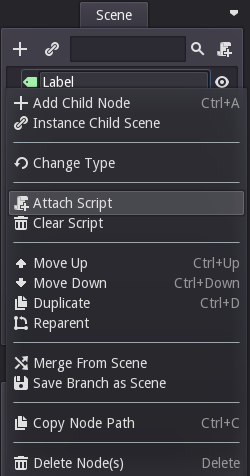
\includegraphics[width=.6\textwidth]{image/editor-attach-script}
    \caption{Opção \textbf{\textit{Attach Script}} para o \textit{node} \textit{Label}}
    \label{editor-attach-script}
  \end{minipage}%
  \begin{minipage}{.5\textwidth}
    \centering
    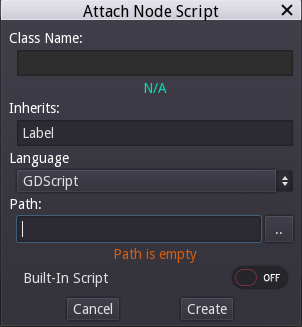
\includegraphics[width=.75\textwidth]{image/editor-script-window}
    \caption{Janela de criação do arquivo \textit{script}}
    \label{editor-script-window}
  \end{minipage}
\end{figure}

Suponha que definimos \textit{Path} como \texttt{res://script.gd} na figura \ref{editor-script-window}. Ao clicarmos em \textit{Create}, a aba central do editor mudará para \textbf{\textit{Script}}, onde o código do arquivo pode ser modificado. Ilustramos a modificação ocorrida na figura \ref{editor-script-write}. Por curiosidade, veja, neste mesma imagem, que todos os recursos (como \textit{scenes}, \textit{scripts} e gráficos) existentes dentro do diretório do projeto são mostrados no canto inferior esquerdo do editor.

\begin{figure}[H]
  \centering
  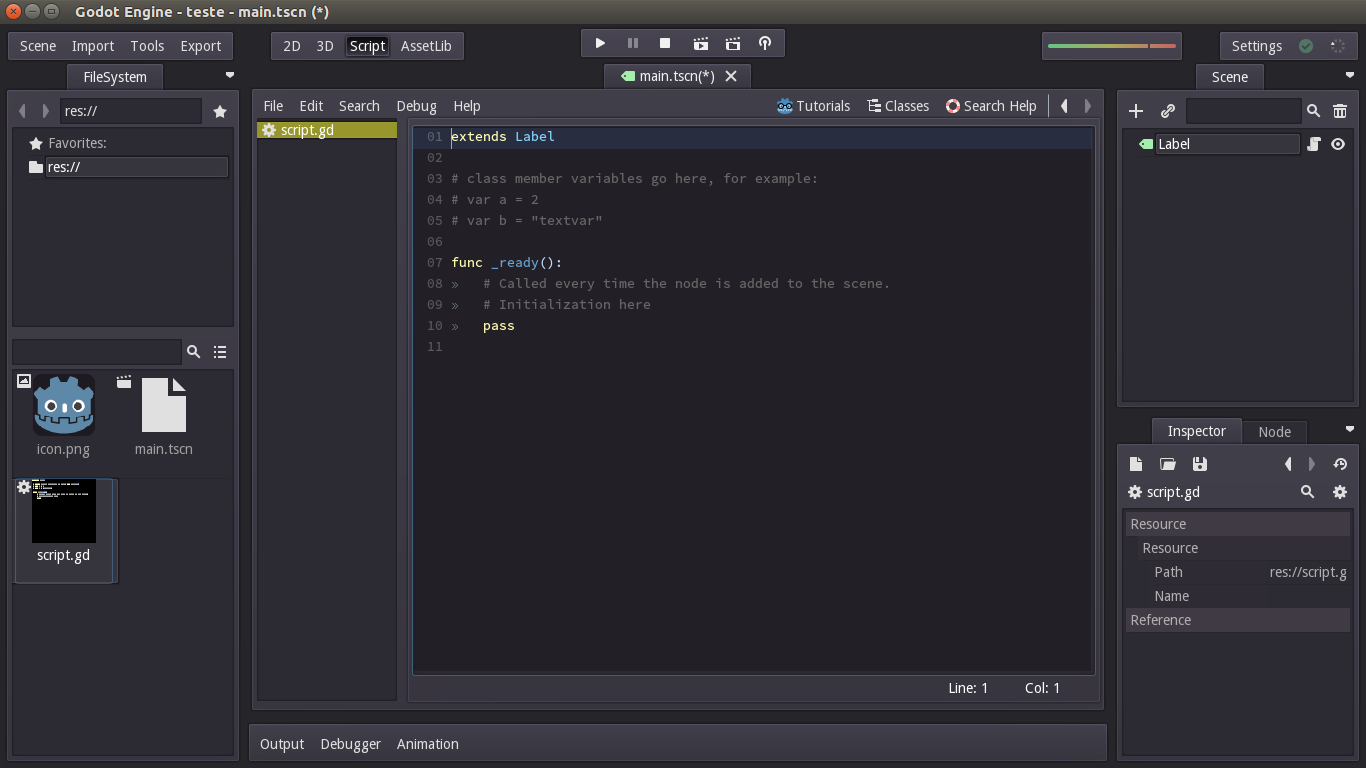
\includegraphics[width=.9\textwidth]{image/editor-script-write}
  \caption{A aba \textbf{\textit{Script}} permite modificar arquivos homônimos}
  \label{editor-script-write}
\end{figure}

Não iremos ensinar, neste trabalho, a linguagem \textit{GDScript} porque o ganho nisso seria mínimo. Um tutorial detalhado, apresentado por \textit{Godot} em \citep{godotGDScriptTutorial}, já existe com esta finalidade. No entanto, explicaremos duas funções predefinidas pela linguagem e que possuem bastante importância no controle de \textit{nodes}.

\subsubsection{\texttt{\_ready()}}

A função \texttt{\_ready()} é chamada sempre que o \textit{node} é adicionado à cena. É geralmente usada para inicializar atributos e preparar configurações de comportamento.

É importante lembrar que nós são organizados em árvore. Portanto, o \texttt{\_ready()} de um \textit{node} pai é sempre chamado antes da função respectiva nos filhos.

\subsubsection{\texttt{\_process(delta)}}

\texttt{\_process()} é uma função chamada repetidamente enquanto o nó existir na cena e \texttt{set\_process(true)} tiver sido chamada previamente (em \_ready(), por exemplo) para solicitar seu uso. Seu único argumento, \texttt{delta}, representa o tempo desde a última atualização de \textit{frame} do jogo.

Esta função é muito útil para executar trechos de código periodicamente durante um jogo. Por exemplo, imagine um jogo em que a personagem controlada pelo usuário possua um certo número de pontos de vida. Poderia-se utilizar \texttt{\_process()} para checar se este valor chegou a zero e, se afirmativo, alterar a \textit{scene} atual para a do fim de jogo.

% ---------------------------------------------------------------------

\section{Planejamento}

Além da escrita de código, jogos costumam usar diversos materiais, ou \emph{assets}, como modelos gráficos, música, sons, fontes e texturas. A criação destes demanda bastante tempo e em geral exige uma equipe diversificada e qualificada. Portanto, gostaríamos de produzir um jogo que utilize poucos \textit{assets}; buscaremos quaisquer materiais necessários em páginas Web que os disponibilizem para uso grátis e sem licença.

Quanto à jogabilidade, desejamos colocar ênfase na funcionalidade de reconhecimento de voz; este é o objetivo em sua criação, afinal. O uso de alguns poucos comandos orais em um jogo curto é o ideal para deixar as regras simples, mas com interação razoável com o usuário.

Por fim, definiremos que o jogo e reconhecimento de voz usarão \textbf{inglês americano} (\textit{US English}), pois sabemos que um modelo acústico e arquivo de dicionário para \textit{Pocketsphinx} existem e são de uso livre para esta língua.

Com estas características em mente, planejamos o jogo \textbf{\emph{Color Clutter}}.

% ---------------------------------------------------------------------

\subsection{Descrição de \textit{Color Clutter}}

Conforme o nome sugere, \textit{Color Clutter} é um jogo cuja temática envolve uma ``confusão'' entre cores.

Uma típica tela do jogo consiste em um fundo totalmente preenchido com alguma cor \(X\). Em alguma posição da tela, uma outra cor \(Y\) aparece escrita em um tom \(Z\). O objetivo do usuário é falar a cor correta (\(X\), \(Y\) ou \(Z\)), de acordo com o que é solicitado em uma legenda apresentada na tela.

Para acrescentar um aspecto competitivo e tornar \textit{Color Clutter} mais lúdico, o jogo será no formato de rodadas, onde marcaremos quantos acertos o usuário consegue em 1 minuto. Cada resposta correta altera aleatoriamente as cores e a posição da palavra na tela; não há penalidade para uma resposta errada, exceto a perda de tempo acarretada pela mesma.

A figura \ref{color-clutter-screen} apresenta a tela do jogo durante uma rodada. O canto superior esquerdo informa qual cor deve ser pronunciada, enquanto o canto superior direito exibem o tempo restante e o \textit{score} (pontuação) atual do jogador. Na situação apresentada, o usuário precisaria falar a cor correspondente ao \textit{background} (fundo): \textbf{\textit{blue}}.

\begin{figure}[H]
  \centering
  \includegraphics[width=.8\textwidth]{image/color-clutter-screen}
  \caption{Tela do jogo \textit{Color Clutter} durante uma rodada}
  \label{color-clutter-screen}
\end{figure}

% ---------------------------------------------------------------------

\section{Desenvolvimento}

A simplicidade de \textit{Color Clutter} nos levou a implementá-lo com apenas uma \textit{scene}. A árvore de \textit{nodes} que o compõe é apresentada na figura \ref{color-clutter-nodes}.

\begin{figure}[H]
  \centering
  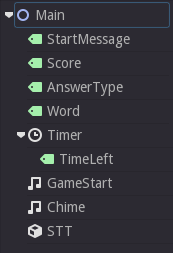
\includegraphics[width=.3\textwidth]{image/color-clutter-nodes}
  \caption{Árvore de \textit{nodes} utilizada em \textit{Color Clutter}}
  \label{color-clutter-nodes}
\end{figure}

Explicamos, a seguir, o funcionamento geral do jogo e detalhamos alguns dos textit{nodes} utilizados.

% ---------------------------------------------------------------------

\subsection{Máquina de estados}

Em termos de funcionamento geral, o jogo transita entre dois estados, \textit{Start} e \textit{Running}. O primeiro caso define o início do jogo, onde espera-se o usuário falar \textit{start} para começar uma partida. Ao reconhecer tal palavra, transita-se para o estado \textit{Running}, correspondente à partida em si, onde o usuário tem 1 minuto para acertar o máximo de cores possíveis. Terminado este tempo, exibe-se a pontuação do jogador e volta-se para o estado \textit{Start}.

A qualquer momento, o usuário pode sair do jogo através do comando de voz \textit{exit}, imediatamente finalizando \textit{Color Clutter}.

% ---------------------------------------------------------------------

\subsection{\textit{Node} \texttt{Main}}

\texttt{Main} é um \textit{Node2D}, que é um nó base para jogos em 2D; por isso seu uso como o \textit{node} raiz da cena.

Conforme indicado na figura \ref{color-clutter-nodes}, este nó contém \texttt{STT}, que é do tipo \textit{STTRunner}. Para poder utilizá-lo, \texttt{Main} prepara dois objetos em \texttt{\_ready()}:

\begin{itemize}
\item Um objeto da classe \textit{STTConfig} (explicado na seção \ref{stt-config}). Definiram-se os arquivos de configuração necessários: um modelo acústico em inglês, um dicionário de palavras em inglês e um arquivo de palavras-chave contendo os comandos usados no jogo. Neste último, os valores de limiar escolhidos foram, em geral, baseados no número de fonemas existentes no comando. Por fim, utilizou-se o método \texttt{init()} para inicializar a instância, deixando-a pronta para uso no \textit{STTRunner}.

\item Um objeto da classe \textit{STTQueue} (explicado na seção \ref{stt-queue}). Esta fila guarda os comandos de voz falados pelo usuário.
\end{itemize}

O laço geral do jogo (\textit{game loop}) está implementado na função \texttt{\_process(delta)}, que é apresentada em pseudocódigo a seguir:

\begin{algorithm}
\begin{algorithmic}[1]
\Function{}{} {\_process}(delta)
\If {\textbf{not} stt\_queue.empty()}
    \State {command $\leftarrow$ stt\_queue.get()}
\EndIf
\State
\If {game\_state == START}
    \If {command == "start"}
        \State {start\_game()}
    \EndIf
\ElsIf {game\_state == RUNNING}
    \If {command == right\_answer}
        \State {update\_score()}
        \State {update\_round()}
    \EndIf
\EndIf
\State
\If {command == "exit"}
    \State {exit\_game()}
\EndIf
\EndFunction
\end{algorithmic}
\end{algorithm}

A função \texttt{update\_score()} é responsável por atualizar a pontuação guardada no \textit{Label} \texttt{Score}, enquanto \texttt{update\_round()} altera os \textit{Labels} \texttt{Word} (a palavra-cor espalhada na tela) e \texttt{AnswerType} (que descreve se a próxima resposta é a palavra, sua cor ou o fundo).

% ---------------------------------------------------------------------

\subsection{\textit{Node} \texttt{Word}}

\texttt{Word} é um nó do tipo \textit{Label}, correspondendo à palavra gerada aleatoriamente pela tela. Quando o usuário acerta a cor da rodada, sua posição é alterada para algum valor dentro dos limites da tela. Garante-se que a cor em que \texttt{Word} é escrita não seja igual à cor de fundo (uma palavra azul em um fundo azul, por exemplo, seria de difícil visualização).

% ---------------------------------------------------------------------

\subsection{\textit{Node} \texttt{Timer}}

\texttt{Timer} é um nó de tipo homônimo. Como o nome indica, ela é usada como um relógio: após atribuir um valor de tempo e acioná-lo, o \textit{Timer} realizará realizar uma contagem regressiva, realizando automaticamente uma chamada de função (\textit{callback}) quando chegar a zero.

No contexto de \textit{Color Clutter}, este \textit{node} automaticamente atualiza seu filho \texttt{TimeLeft}, que é um \textit{Label} usado para indicar, na tela, o  tempo restante de jogo. \texttt{Timer} chama uma função em \texttt{Main} quando a partida acaba, com o objetivo de alterar o estado do jogo para \textit{Start}.

% ---------------------------------------------------------------------

\subsection{\textit{Nodes} \texttt{GameStart} e \texttt{Chime}}

\texttt{GameStart} e \texttt{Chime} são nós do tipo \textit{StreamPlayer}. Guardam um efeito sonoro tocado no início do jogo e quando o usuário acerta a cor, respectivamente.

% ---------------------------------------------------------------------

\section{Testes}

\textit{Color Clutter} foi testado por 10 pessoas com boa fluência em inglês. A maioria dos testadores utilizavam alguma versão de \textit{Windows} (versões 7, 8 ou 10), com três testes sendo feitos nas distribuições \textit{Ubuntu}, \textit{Debian} e \textit{Linux Mint} do sistema operacional \textit{Unix}.

Um dos primeiros resultados visualizados é que não houve diferença perceptível no reconhecimento de voz execução entre os sistemas operacionais. Todos os testadores comentaram que a velocidade de reconhecimento estava rápida (menos de 1 segundo).

No entanto, praticamente todas as pessoas envolvidas no teste comentaram que alguns comandos não eram reconhecidos na primeira vez em que eram pronunciados, exigindo-se repeti-los 2 ou 3 vezes até serem aceitos. Destacam-se as cores \textit{green}, \textit{orange} e \textit{purple} como as palavras que, em geral, geravam maior dificuldade de reconhecimento.

A efeito de comparação, executou-se uma API de reconhecimento de voz desenvolvida pelo Google \citep{googleSpeechAPI}, configurada para o inglês americano, simultaneamente em que \textit{Color Clutter} era jogado. Este programa reconheceu todas as palavras proferidas enquanto \textit{Color Clutter}, por vezes, não entendia algum comando. Duas respostas possíveis surgem para esta diferença: a eficiência da API do Google é bem maior do que a de \textit{Pocketsphinx}, ou é necessário um ajuste no limiar das palavras-chave do jogo (isto é, é possível que uma pronúncia muito parecida com a da fonética do dicionário esteja sendo exigida).

% ---------------------------------------------------------------------

\section{Divulgação}

Todo o código fonte do projeto \textit{Color Clutter} encontra-se em um repositório no GitHub do autor \citep{colorClutterGitHub}, juntamente com as instruções do jogo. Também foram disponibilizados binários para \textit{Windows} e \textit{Unix} \citep{colorClutterDownload}.

\textit{Color Clutter} foi divulgado nos mesmos dois fóruns de \textit{Godot} onde publicou-se sobre \textit{Speech to Text}:

\begin{itemize}
\item \textbf{Godot Engine Q\&A} \citep{colorClutterGodotQA}: Embora não seja mais voltado para tirar dúvidas, publicou-se o jogo no site oficial de \textit{Godot}.

\item \textbf{Godot Developers} \citep{colorClutterGodotDevelopers}: Voltado principalmente para jogos produzidos na \textit{game engine}.
\end{itemize}

\chapter{Conclusão}
\label{cap:conclusion}

Este Trabalho de Conclusão de Curso envolveu o desenvolvimento de um módulo de reconhecimento de voz para a \textit{game engine} \textit{Godot}. Para tanto, dedicou-se um tempo razoável do trabalho para o estudo das principais características de sistemas de reconhecimento de voz. Ficou evidente o vasto uso que esta tecnologia possui hoje, e o futuro indica que seu uso poderá crescer ainda mais. A tendência de ideologias como \emph{Internet das Coisas} é trazer cada vez mais poder computacional para automatizar tarefas repetitivas na vida do ser humano, e interação por voz se encaixaria bem para tais situações.

A procura por bibliotecas de código aberto que atendam a certas expectativas veio a seguir, levando-nos a estudar \textit{Pocketsphinx} como a opção mais viável no contexto de usabilidade dentro de um jogo. Apesar da documentação da biblioteca ser por vezes incompleta, vários exemplos em fóruns possibilitaram um aprendizado satisfatório de seu uso.

\textit{Godot} possui uma documentação bastante completa quanto a seu uso para jogos. No entanto, não há muito material disponível relacionado a suas classes em \textit{C++}. A leitura e entendimento de código, portanto, foi uma habilidade bastante exercida nesta parte, uma vez que certas implementações no módulo \textit{Speech to Text} foram baseadas em algo já feito em outra classe.

A produção do pequeno jogo \textit{Color Clutter} teve importância considerável no final deste trabalho, pois mostrou que o módulo correspondeu às expectativas referentes a eficiência e simplicidade de uso.

Em geral, o resultado final foi bastante satisfatório, uma vez que o módulo \textit{Speech to Text} foi até divulgado, com seu código aberto, em fóruns da \textit{game engine}, junto ao jogo \textit{Color Clutter} produzido. Deseja-se continuar o suporte ao módulo no futuro, possivelmente estudando-se mais sobre \textit{Android} e \textit{MacOS} para tentar portá-lo a estes sistemas operacionais.


{
\fancyhead[RO]{\nouppercase{Agradecimentos}}
\fancyhead[LE]{\nouppercase{Agradecimentos}}
\fancyhead[RE,LO]{}
\chapter*{Agradecimentos}
\addcontentsline{toc}{chapter}{Agradecimentos}

Gostaria de agradecer muito a minha família, principalmente meus pais, pelo constante apoio durante toda a minha vida universitária. Dificilmente teria conseguido arranjar forças para chegar até o final do curso se não fosse por eles.

Sou muito grato ao IME e aos professores com as quais tive aula. Pretendo levar a dedicação e ensinamentos deles pelo resto de minha vida profissional. Em especial, agradeço ao meu orientador, o professor Gubi, pelas várias reuniões e conversas ao longo do ano sobre este trabalho.

Por fim, agradeço o apoio dos poucos mas valiosos amigos que fiz durante a graduação, pois a experiência da universidade não teria sido a mesma sem a presença deles.

}

{
\fancyhead[RO]{\nouppercase{Disciplinas importantes para este trabalho}}
\fancyhead[LE]{\nouppercase{Disciplinas importantes para este trabalho}}
\fancyhead[RE,LO]{}
\chapter*{Disciplinas importantes para este trabalho}
\addcontentsline{toc}{chapter}{Disciplinas importantes para este trabalho}

Dentre as disciplinas que cursei durante a graduação, as seguintes se destacam pela relação maior com a confecção deste trabalho:

\subsubsection{(MAC0110) Introdução a Computação \\
(MAC0122) Princípios de Desenvolvimento de Algoritmos \\
(MAC0323) Estrutura de Dados}

Entrei no Bacharelado em Ciência da Computação sem conhecimento algum de programação, mas com o intuito de aprender bastante sobre o assunto. Estas três disciplinas fornecerem a base poderosa que eu desejava, e mostraram que programar não é apenas redigir código. Escrever um programa eficiente, robusto e correto exige raciocínio lógico, capacidade de abstração e domínio das estruturas de dados disponíveis.

\subsubsection{(MAC0211) Laboratório de Programação I \\
(MAC0242) Laboratório de Programação II}

Estas disciplinas possuem um foco mais prático de ferramentas e concepções para programação em si. Destacam-se o uso de linguagens de \textit{script}, expressões regulares e Programação Orientada a Objetos. Meu primeiro contato com \textit{UML} também ocorreu nestas disciplinas.

\subsubsection{(MAC0332) Engenharia de Software}

Apresentou metodologias interessantes para a produção de software. Também tive um forte contato com diagramas \textit{UML}. Sinto que a classificação de software de acordo com sua finalidade e técnicas importantes para planejamento me ajudou, de certa forma, na preparação dos requisitos do módulo de reconhecimento de voz.

\subsubsection{(MAC0441) Programação Orientada a Objetos}

Primeira experiência com a produção de um \textit{software} de proporção maior que um Exercício-Programa, pois fora realizado um projeto sobre Cidades Inteligentes que englobou a classe inteira. Ajudou a aprofundar meus conhecimentos sobre Orientação a Objetos e a produção de código de qualidade.

\subsubsection{(MAC0422) Sistemas Operacionais}

Apresentou a ideia de \textit{threads} pela primeira vez no curso, além de mostrar as componentes principais de sistemas operacionais. Em especial, destacamos o gerenciamento de arquivos, que apareceu, neste trabalho, na implementação própria do sistema de arquivos de \textit{Godot}.

\subsubsection{(MAC0425) Inteligência Artificial}

Alguns tópicos, como \textit{Markov Decision Process} (MDP), lembram o procedimento estocástico comentado em \textit{Hidden Markov Model} (HMM).

}

% ---------------------------------------------------------------------
% Appendix

% Header
\renewcommand{\chaptermark}[1]{\markboth{\MakeUppercase{\appendixname\ \thechapter}} {\MakeUppercase{#1}} }
\fancyhead[RE,LO]{}
\appendix

% Add appendix files here

% ---------------------------------------------------------------------
% Bibliography

\backmatter
\bibliographystyle{bib/plainnat-ime}  % Textual bibliographic quote

% Header for bibliography pages
\fancyhead[RO]{\nouppercase{\rightmark}}
\fancyhead[LE]{\nouppercase{\leftmark}}
\fancyhead[RE,LO]{}

% Add bibliography files here
\bibliography{bib/stt-theory,bib/stt-libs,bib/godot,bib/other}

% ---------------------------------------------------------------------

\end{document}
